% \documentclass[dvipdfmx, a4paper, 11pt]{jsarticle}%A4用紙縦,明朝(デフォルト)11ポイント
\documentclass[dvipdfmx,titlepage, 11pt, a4paper]{jsarticle}%A4用紙縦,明朝(デフォルト)11ポイント
\usepackage[top=18truemm,bottom=18truemm,left=18truemm,right=18truemm]{geometry}%余白調整
% \setlength{\textheight}{45\baselineskip}
% \setlength{\textwidth}{46zw}% 46文字/行

\usepackage{template}

%%%====================================================================================================================================
\renewcommand{\thesection}{第\arabic{section}問}
\renewcommand{\thesubsection}{\thesection}
\titleformat*{\section}{\LARGE\mcfamily}%章のタイトルの文字の大きさを通常サイズに設定(明朝体で)
\titlespacing*{\section}{0pt}{*0}{0pt}%章番号の後の空白行の削除
\titleformat*{\subsection}{\Large\mcfamily}%節のタイトルの文字の大きさを通常サイズに設定(明朝体で)
\titlespacing*{\subsection}{0pt}{*0}{0pt}%節番号の後の空白行の削除
\titleformat*{\subsubsection}{\large\mcfamily}%小節のタイトルの文字の大きさを通常サイズに設定(明朝体で)
\titlespacing*{\subsubsection}{0pt}{*0}{0pt}%小節番号の後の空白行の削除

\makeatletter
%章番号付きコード番号
\AtBeginDocument{
  \renewcommand*{\thelstlisting}{\arabic{section}.\arabic{lstlisting}}%
  \@addtoreset{lstlisting}{section}
}

%章番号付き表番号
\renewcommand{\thetable}{%
    \arabic{section}.\arabic{table}%
}
\@addtoreset{table}{section}%

%章番号付き図番号
\renewcommand{\thefigure}{%
	\arabic{section}.\arabic{figure}%
}%
\@addtoreset{figure}{section}%

%章番号付き式番号
\renewcommand{\theequation}{%
	\arabic{section}.\arabic{equation}%
}%
\@addtoreset{equation}{section}%

\renewcommand{\p@enumiii}{}% 箇条書きの参照時の番号の変更(2(親の番号)a(子の番号)→aだけに)
\renewcommand{\p@enumii}{}% 箇条書きの参照時の番号の変更(2a→aだけに)
\makeatother
%%%====================================================================================================================================

%%%====================================================================================================================================
%%ページのレイアウト設定
\pagestyle{fancy}
\renewcommand{\sectionmark}[1]{\markboth{}{\thesection\ #1}}%                   %\rightmarkにセクション名を格納
\renewcommand{\subsectionmark}[1]{\markboth{#1}{\rightmark}}%   %\leftmarkにサブセクション名を格納
%[]は省略可で省略すると{}で指定された内容が偶数ページ奇数のどちらにも適用される.
% \renewcommand{\headrulewidth}{0pt} %ヘッダの罫線を消す 
\fancyfoot{}%                        %clear all footer fields
\lhead{\leftmark}%                   %左側ヘッダの定義[<偶数ページ>]{<奇数ページ>}
\chead{}%                            %中央ヘッダの定義[<偶数ページ>]{<奇数ページ>}
\rhead{\rightmark}%                  %右側ヘッダの定義[<偶数ページ>]{<奇数ページ>}
\lfoot{東大2019年度数学解答例}%       %左側フッターの定義[<偶数ページ>]{<奇数ページ>}
\cfoot{\thepage}%                    %中央フッターの定義[<偶数ページ>]{<奇数ページ>}
\rfoot{文殊の知恵}%                  %右側フッターの定義[<偶数ページ>]{<奇数ページ>}
\renewcommand{\headrulewidth}{0.1pt}%%ヘッダの線の太さ 
\renewcommand{\footrulewidth}{0.1pt}%%フッターの線の太さ
%%%====================================================================================================================================

\makeindex%索引用

\renewcommand{\refname}{}%参考文献の文字を非表示にする
\title{\Huge 東大2019年度数学解答例\\[10mm]}
\author{{\LARGE 文殊の知恵}\\[1mm]\LARGE 高橋那弥\\(加筆:中田昌輝)}
\date{}

\begin{document}
\maketitle
\tableofcontents % 目次
\pagenumbering{roman}%目次のページ番号のスタイルをローマ数字にする
\newpage
\setcounter{tocdepth}{3}%章節の深さを3にするsubsubsectionまで
\pagenumbering{arabic}%他のページ番号は通常の数字にする.
\section{}%第1問
\subsection{問題文}
複素正方行列$X$は$XX^{\ast}=I$を満たすとき,ユニタリ行列であるという.但し,$X^{\ast}$は行列$X$の共役転置行列(もしくは随伴行列)を
表し,$I$は単位行列とする.また,iは虚数単位とする.以下の問いに答えよ.
\begin{enumerate}[(1)]
    \setlength{\itemsep}{10pt}
    \item $n$を正の整数とし,$A, B$を$n$次ユニタリ行列とする.行列$AB$もユニタリ行列であることを示せ.
    \item $n$を正の整数とし,$C, D$を$n$次実正方行列とする.行列$F$を$F = C + \imag D$と定義し,行列$G$を
    \begin{align*}
        G = \spalignmat{
            C {-D};
            D {C}
        }
    \end{align*}
    と定義する.行列$F$がユニタリ行列であることと行列$G$が直交行列であることは同値であることを示せ.
    \item 次の行列の固有値を求めよ.
    \begin{align*}
        \frac{1}{2}\spalignmat{
            1 1 1 1;
            1 {\imag} -1 {-\imag};
            1 -1 1 -1;
            1 {-\imag} -1 {\imag}
        }
    \end{align*}
    \item $n$を正の整数とし,$n$次正方行列$Q$の$(j, k)$成分$q_{jk}$を
    \begin{equation*}
        q_{jk} = \cfrac{1}{\sqrt{n}}\exp \left(\cfrac{2\pi\imag (j - 1)(k - 1)}{n}\right)
    \end{equation*}
    とする.行列$Q$はユニタリ行列であることを示せ.
    \item 行列式が1である2次のユニタリ行列は次の一形式を持つことを示せ.但し,$\theta, \psi$は実数であるとする. (これは一般形ではないので, 誤植修正しました).
    \begin{equation*}
        H = \spalignmat{
            {\exp(\imag \psi_{1})\cos\theta} {\exp(\imag \psi_{2})\sin\theta};
            {-\exp(-\imag \psi_{2})\sin\theta} {\exp(-\imag \psi_{1})\cos\theta}
        }
    \end{equation*}
    \item 2次のユニタリ行列の一般形を求めよ
\end{enumerate}

\newpage

\subsection{解答例}
\begin{enumerate}[(1)]
    \setlength{\itemsep}{10pt}
    \item $A, B$ともにユニタリ行列より以下が成り立つ.
    \begin{align}
        \left\{
            \begin{array}{lcl}
            AA^{\ast} &=& I\\ 
            BB^{\ast} &=& I\\ 
            \end{array}
        \right.\label{eq:abunitary}
    \end{align}
    よって,式\eqref{eq:abunitary}より,以下が成り立つ.
    \begin{align*}
        (AB)(AB)^{\ast} & = ABB^{\ast}A^{\ast}\\
                        & = AIA^{\ast}\\
                        & = AA^{\ast}\\
                        & = I
    \end{align*}
    よって,行列$AB$についてもユニタリ行列であることが示された.
    \item 題意は以下のように同値変形できる.
    \begin{align}
        \mbox{行列$F$がユニタリ行列であること}&\mbox{と行列$G$が直交行列であることは同値である}\nonumber\\
        \Longleftrightarrow \mbox{行列$F$がユニタリ行列である} &\Leftrightarrow \mbox{行列$G$が直交行列である} \nonumber\\
        \Longleftrightarrow FF^{\ast} = I &\Leftrightarrow GG^{\top} = I\label{eq:hodai1_2}
    \end{align}
    よって,式\eqref{eq:hodai1_2}が成り立つことを示せばよい.

    まず以下の式\eqref{eq:hodai1_2_1}が成り立つことを示す.
    \begin{equation}
        FF^{\ast} = I \Rightarrow GG^{\top} = I \label{eq:hodai1_2_1}
    \end{equation}
    題意より,$F = C + \imag D$より,$F^{\ast} = C^{\top} - \imag D^{\top}$であり,
    式\eqref{eq:hodai1_2_1}の仮定条件$FF^{\ast} = I$から以下が成り立つ.
    \begin{align*}
        FF^{\ast} & = \left(C + \imag D\right)\left(C^{\top} - \imag D^{\top}\right)\\
                & = CC^{\top} + DD^{\top} + \imag \left(DC^{\top} - CD^{\top}\right)\\
                & = I\\
        \Longleftrightarrow
        I & = CC^{\top} + DD^{\top} + \imag \left(DC^{\top} - CD^{\top}\right)\\
        \Longrightarrow I&\mbox{は実正方行列より} \mbox{\boldmath $0$} = DC^{\top} - CD^{\top}\\
        \Longrightarrow I & = CC^{\top} + DD^{\top}\\
        \therefore GG^{\top} & = 
        \spalignmat{
            C {-D};
            D {C}
        }
        \spalignmat{
            {C^{\top}} {D^{\top}};
            {-D^{\top}} {C^{\top}}
        }\\
        & = 
        \spalignmat{
            {CC^{\top} + DD^{\top}} {CD^{\top} - DC^{\top}};
            {DC^{\top} - CD^{\top}} {DD^{\top} + CC^{\top}}
        }\\
        & = 
        \spalignmat{
            {I} {\mbox{\boldmath $0$}};
            {\mbox{\boldmath $0$}} {I}
        }\\
        & = I
    \end{align*}
    よって,式\eqref{eq:hodai1_2_1}が成り立つことは示された.

    次に以下の式\eqref{eq:hodai1_2_2}が成り立つを示す.
    \begin{equation}
        GG^{\top} = I \Rightarrow FF^{\ast} = I \label{eq:hodai1_2_2}
    \end{equation}
    題意と式\eqref{eq:hodai1_2_2}の仮定条件$GG^{\top} = I$から以下が成り立つ.
    \begin{align*}
        GG^{\top} & = 
        \spalignmat{
            C {-D};
            D {C}
        }
        \spalignmat{
            {C^{\top}} {D^{\top}};
            {-D^{\top}} {C^{\top}}
        }\\
        & = 
        \spalignmat{
            {CC^{\top} + DD^{\top}} {CD^{\top} - DC^{\top}};
            {DC^{\top} - CD^{\top}} {DD^{\top} + CC^{\top}}
        }\\
        & = I\\
        \Longleftrightarrow &
        \begin{cases}
            \mbox{\boldmath $0$} = CD^{\top} - DC^{\top}\\
            I = CC^{\top} + DD^{\top}
        \end{cases}
    \end{align*}
    \begin{align*}
        \therefore FF^{\ast} & = \left(C + \imag D\right)\left(C^{\top} - \imag D^{\top}\right)\\
            & = CC^{\top} + DD^{\top} + \imag \left(DC^{\top} - CD^{\top}\right)\\
            & = I + \mbox{\boldmath $0$}\\
            & = I
    \end{align*}
    よって,式\eqref{eq:hodai1_2_2}が成り立つことが示された.

    従って,式\eqref{eq:hodai1_2_1}, \eqref{eq:hodai1_2_2}が成り立つことが示されたので,式\eqref{eq:hodai1_2}
    が成り立つことが示された.よって,題意は示された.\\[1cm]
    (中田解)
    \begin{eqnarray*}
    行列Fがユニタリ行列である&\Longleftrightarrow&FF^{*}=I\\
                            &\Longleftrightarrow&(C+{\rm i}D)(C+{\rm i}D)^{*}=I\\
                            &\Longleftrightarrow&(C+{\rm i}D)(C^{\sf T}-{\rm i}D^{\sf T})=I\\
                            &\Longleftrightarrow&(CC^{\sf T}+DC^{\sf T})+{\rm i}(DC^{\sf T}+CD^{\sf -T})=I\\
                            &\Longleftrightarrow&\left\{\begin{array}{l}CC^{\sf T}+DD^{\sf T}=I\\DC^{\sf T}+CD^{\sf T}=\bm{0}\end{array}\right.\\
                            &\Longleftrightarrow&\begin{pmatrix}CC^{\sf T}+DD^{\sf T}&\bm{0}\\\bm{0}&CC^{\sf T}+DD^{\sf T}\end{pmatrix}=I\\
                            &\Longleftrightarrow&\begin{pmatrix}C&-D\\D&C\end{pmatrix}\begin{pmatrix}C^{\sf T}&D^{\sf T}\\-D^{\sf T}&C^{\sf T}\end{pmatrix}=I\\
                            &\Longleftrightarrow&GG^{\sf T}=I
    \end{eqnarray*}
    よって, 題意は示された.
    \item 題意の4次正方行列を$A$とおき,$\mid A \mid$は行列$A$の行列式を表すとすると,
    固有値$\lambda$は以下を満たす.
    \begin{equation*}
        \mid \lambda I - A \mid = 0
    \end{equation*}
    よって,この方程式を解くと以下のようになる.
    \begin{align*}
        \mid \lambda I - A \mid 
        & = \left(\frac{1}{2}\right)^{4} \mid 2\lambda I - 2A \mid\\
        & = \frac{1}{16}
        \spaligndelims\vert\vert \spalignmat{
            {2\lambda - 1} -1 -1 -1;
            -1 {2\lambda - \imag} 1 {\imag};
            -1 1 {2\lambda - 1} 1;
            -1 {\imag} 1 {2\lambda - \imag}
        }\\
        & = \frac{1}{16}
        \spaligndelims\vert\vert \spalignmat{
            0 {(2\lambda - 1)(2\lambda - \imag) - 1} {2\lambda - 2} {\imag(2\lambda - 1) - 1};
            -1 {2\lambda - \imag} 1 {\imag};
            0 {1 + \imag - 2\lambda} {2\lambda - 2} {1 - \imag};
            0 {2\imag - 2\lambda} 0 {2\lambda - 2\imag}
        }\\
        & = \frac{1}{16}\times (-1)^{2 + 1}\times (-1)
        \spaligndelims\vert\vert \spalignmat{
            {(2\lambda - 1)(2\lambda - \imag) - 1} {2\lambda - 2} {\imag(2\lambda - 1) - 1};
            {1 + \imag - 2\lambda} {2\lambda - 2} {1 - \imag};
            {2\imag - 2\lambda} 0 {2\lambda - 2\imag}
        }\\
        & = \frac{1}{16}
        \spaligndelims\vert\vert \spalignmat{
            {(2\lambda - 1)(2\lambda - \imag) - 1} {2\lambda - 2} {2\lambda(2\lambda - 1) - 2};
            {1 + \imag - 2\lambda} {2\lambda - 2} {2 - 2\lambda};
            {2\imag - 2\lambda} 0 0
        }\\
        & = \frac{1}{16}\times (-1)^{3 + 1} \times (2\imag - 2\lambda)
        \spaligndelims\vert\vert \spalignmat{
            {2\lambda - 2} {2\lambda(2\lambda - 1) - 2};
            {2\lambda - 2} {2 - 2\lambda}
        }\\
        & = \frac{1}{16}(2\imag - 2\lambda)(2\lambda - 2)\left[2 - 2\lambda - \left\{2\lambda(2\lambda - 1) - 2\right\}\right]\\
        & = \frac{1}{2}(\imag - \lambda)(\lambda - 1)(2 - \lambda - 2\lambda^2 + \lambda)\\
        & = (\imag - \lambda)(\lambda - 1)(1 - \lambda^2)\\
        & = (\lambda - \imag)(\lambda - 1)^2(\lambda + 1)\\
        \therefore\, \lambda & = \pm 1, \imag
    \end{align*}
    よって,固有値は$\pm 1 \imag$である.\\[1cm]
    (中田解)\\
    この行列を$A$とし, この行列$A$に対する固有値を$\lambda$, 固有ベクトルを$\bm{x}$とおくと
    \begin{eqnarray*}
        A\bm{x} = \lambda\bm{x} &\Longleftrightarrow& (\lambda I -A)\bm{x} = \bm{0}\\
                                &\Longleftrightarrow& {\rm det}|\lambda I-A|=0
    \end{eqnarray*}
    が成り立つ. ゆえに求める固有値$\lambda$は
    \begin{eqnarray*}
        && \mathrm{det}\left\lvert
        \begin{pmatrix}
            \lambda & 0 & 0 & 0\\
            0 & \lambda & 0 & 0\\
            0 & 0 & \lambda & 0\\
            0 & 0 & 0 & \lambda 
        \end{pmatrix}
        -\frac{1}{2}
        \begin{pmatrix}
            1 & 1 & 1 & 1\\
            1 & \imag & -1 & -\imag\\
            1 & -1 & 1 & -1\\
            1 & -\imag & -1 & \imag
        \end{pmatrix}
        \right\rvert = 0\\
        \Longleftrightarrow\ && \mathrm{det}\left\lvert
        \frac{1}{2}
        \begin{pmatrix}
            2\lambda - 1 & -1 & -1 & -1\\
            -1 & 2\lambda - \imag & 1 & \imag\\
            -1 & 1 & 2\lambda - 1 & 1\\
            -1 & \imag & 1 & 2\lambda - \imag
        \end{pmatrix}\right\rvert = 0\\
        \Longleftrightarrow\ && 
        \begin{vmatrix}
            2\lambda - 1 & -1 & -1 & -1\\
            -1 & 2\lambda - \imag & 1 & \imag\\
            -1 & 1 & 2\lambda - 1 & 1\\
            -1 & \imag & 1 & 2\lambda - \imag
        \end{vmatrix} = 0\\
        \Longleftrightarrow\ && 
        \begin{vmatrix}
            0 & -1 + (2\lambda - 1)(2\lambda - \imag) & 2\lambda - 2 & -1 + \imag(2\lambda - 1)\\
            -1 & 2\lambda - \imag & 1 & \imag\\
            0 & -2\lambda + \imag + 1 & 2\lambda - 2 & 1 - \imag\\
            0 & -2\lambda + 2\imag & 0 & 2\lambda - 2\imag
        \end{vmatrix} = 0\\
        \Longleftrightarrow\ && 
        \begin{vmatrix}
            -1 + (2\lambda - 1)(2\lambda - \imag) & 2\lambda - 2 & -1 + \imag(2\lambda - 1)\\
            -2\lambda + \imag + 1 & 2\lambda - 2 & 1 - \imag\\
            -2\lambda + 2\imag & 0 & 2\lambda - 2\imag
        \end{vmatrix} = 0\\
        \Longleftrightarrow\ && 
        \begin{vmatrix}
            -1 + (2\lambda - 1)(2\lambda - \imag) & 2\lambda - 2 & -2 + 2\lambda(2\lambda - 1)\\
            -2\lambda + \imag + 1 & 2\lambda - 2 & -2\lambda + 2\\
            -2\lambda + 2\imag & 0 & 0
        \end{vmatrix} = 0\\
        \Longleftrightarrow\ && (-2\lambda + 2\imag)
        \begin{vmatrix}
            2\lambda - 2 & -2 + 2\lambda(2\lambda - 1)\\
            2\lambda - 2& -2\lambda + 2
        \end{vmatrix} = 0\\
        \Longleftrightarrow\ && (\lambda - \imag)(\lambda - 1)
        \begin{vmatrix}
            1 & -2 + 2\lambda(2\lambda - 1)\\
            1 & -2\lambda + 2
        \end{vmatrix} = 0\\
        \Longleftrightarrow\ && (\lambda - \imag)(\lambda - 1)\bigl\{-2\lambda + 2 + 2 - 2\lambda(2\lambda - 1)\bigr\} = 0\\
        \Longleftrightarrow\ && (\lambda - \imag)(\lambda - 1)(-4\lambda^{2} + 4) = 0\\
        \Longleftrightarrow\ && (\lambda - \imag)(\lambda - 1)(\lambda^{2} - 1) = 0\\
        \Longleftrightarrow\ && (\lambda - \imag)(\lambda - 1)^{2}(\lambda + 1) = 0\\
        \Longleftrightarrow\ && \lambda = \pm 1,\imag
    \end{eqnarray*}
    よって, 固有値は$\pm 1,\ \imag$である.\\
    \underline{中田別方針}\\
    問題の行列を$A$とすると
    \begin{eqnarray*}
        AA^{\ast}=I
    \end{eqnarray*}
    より,$A$はユニタリ行列である. この$A$の固有値を$\lambda$, 固有ベクトルを$\bm{x}$とすると
    \begin{eqnarray*}
        A\bm{x}=\lambda \bm{x}
    \end{eqnarray*}
    が成り立ち, 複素内積と随伴行列の間に
    \begin{eqnarray*}
        \langle \bm{x},A\bm{y}\rangle = \langle A^{\ast}\bm{x},\bm{y}\rangle
    \end{eqnarray*}
    の関係があることから
    \begin{eqnarray*}
        \langle A\bm{x},A\bm{x}\rangle &=& \langle A^{\ast}A\bm{x},\bm{x}\rangle\\
                                       &=&\langle \bm{x},\bm{x}\rangle\\
                                       &=&\|\bm{x}\|^{2}
    \end{eqnarray*}
    となり, $A\bm{x}$同士の内積は$\bm{x}$のノルムの2乗に等しくなる.\\
    一方で, 複素内積の性質で
    \begin{eqnarray*}
        \langle \bm{x},\alpha \bm{y}\rangle &=& \alpha \langle \bm{x},\bm{y}\rangle \\
        \langle \alpha \bm{x},\bm{y}\rangle &=& \alpha^{\ast}\langle \bm{x},\bm{y}\rangle
    \end{eqnarray*}
    となるので,
    \begin{eqnarray*}
        \langle A\bm{x},A\bm{x}\rangle &=& \langle \lambda \bm{x},\lambda \bm{x}\rangle \\
                                       &=&\lambda^{\ast}\langle \bm{x},\lambda \bm{x}\rangle\\
                                       &=& \lambda^{\ast}\lambda \langle \bm{x},\bm{x}\rangle\\
                                       &=&|\lambda|^{2}\|\bm{x}\|^{2}
    \end{eqnarray*}
    したがって,
    \begin{eqnarray*}
      \|\bm{x}\|^{2} = |\lambda|^{2}\|\bm{x}\|^{2}
    \end{eqnarray*}
    ここで, $\bm{x}\neq \bm{0}$から$\|\bm{x}\|^{2}\neq 0$であるので,
    \begin{eqnarray*}
      |\lambda|^{2} = 1\Longleftrightarrow |\lambda| = 1
    \end{eqnarray*}
    となる. 4次のユニタリ行列であるので, $\lambda =\pm 1,\pm \imag$が候補に上がる. これから固有ベクトルを求めて一致するかどうかを確認する.
    \item 題意より複素数$z$に対する共役な複素数を$\overline{z}$と表すとき,
    $n$次正方行列$Q$の共役転置行列$Q^{\ast}$の$(j, k)$成分$q^{\ast}_{jk}$は以下のようになる.
    \begin{align}
        q^{\ast}_{jk} & = \overline{q_{kj}}\nonumber\\
        & = \cfrac{1}{\sqrt{n}}\exp \left(\cfrac{-2\pi\imag (k - 1)(j - 1)}{n}\right)\label{eq:kyoyaku}
    \end{align}
    よって,式\eqref{eq:kyoyaku}から$QQ^{\ast}$の$(j, k)$成分$Q_{jk}$は以下のようになる.
    \begin{align*}
        Q_{jk} & = \sum_{l = 1}^{n} \left(q_{jl}\times q^{\ast}_{lk}\right)\\
               & = \sum_{l = 1}^{n}
               \left\{
               \cfrac{1}{\sqrt{n}}\exp \left(\cfrac{2\pi\imag (j - 1)(l - 1)}{n}\right)
               \times 
               \cfrac{1}{\sqrt{n}}\exp \left(\cfrac{-2\pi\imag (k - 1)(l - 1)}{n}\right)
               \right\}\\
               & = \cfrac{1}{n} \sum_{l = 1}^{n}
               \exp\left(\cfrac{2\pi\imag (j - 1)(l - 1)}{n} + \cfrac{-2\pi\imag (k - 1)(l - 1)}{n}\right)\\
               & = \cfrac{1}{n} \sum_{l = 0}^{n - 1}
               \exp\left(\cfrac{2\pi\imag (j - k)l}{n}\right)\\
               & = 
               \begin{cases}
                \cfrac{1}{n}\sum\limits_{l = 0}^{n - 1}\exp(0) & j = k\\
                &\\
                \cfrac{1}{n}\cfrac{\exp\left(\cfrac{2\pi\imag (j - k)n}{n}\right) - \exp(0)}{\exp\left(\cfrac{2\pi\imag (j - k)}{n}\right) - 1}& j \neq k
               \end{cases}\\
        \mbox{オイラーの公式から}&j, k\mbox{は整数より}\\
        Q_{jk} & = 
        \begin{cases}
            1 & j = k\\
            \cfrac{1}{n}\cfrac{\cos\{2\pi(j - k)\} + \imag \sin\{2\pi(j - k)\} - 1}{\exp\left(\cfrac{2\pi\imag (j - k)}{n}\right) - 1} = 0 & j \neq k
        \end{cases}
    \end{align*}
    従って,対角成分のみ1となり,他の成分は全て0となるので,$QQ^{\ast}$は単位行列となる.従って,$Q$はユニタリ行列であることが示された.
    \item 題意の2次正方行列$H$についてユニタリ行列であることを示す.
    \begin{align*}
        HH^{\ast} & = 
        \spalignmat{
            {\exp(\imag \psi)\cos\theta} {\exp(\imag \psi)\sin\theta};
            {-\exp(-\imag \psi)\sin\theta} {\exp(-\imag \psi)\cos\theta}
        }
        \spalignmat{
            {\exp(-\imag \psi)\cos\theta} {-\exp(\imag \psi)\sin\theta};
            {\exp(-\imag \psi)\sin\theta} {\exp(\imag \psi)\cos\theta}
        }\\
        & = 
        \spalignmat{
            {\exp(\imag \psi - \imag \psi)(\cos^{2}\theta + \sin^{2}\theta)} 
            {\exp(2\imag \psi)(-\cos\theta\sin\theta + \sin\theta\cos\theta)};
            {\exp(-2\imag \psi)(-\sin\theta\cos\theta + \cos\theta\sin\theta)} 
            {\exp(-\imag \psi + \imag \psi)(\sin^{2}\theta + \cos^{2}\theta)}
        }\\
        & = 
        \spalignmat{
            {1} {0};
            {0} {1}
        }\\
        & = I
    \end{align*}
    よって,行列$H$はユニタリ行列である.また,行列$H$の行列式は以下のようになる.
    \begin{align*}
        \mid H \mid & = \exp(\imag \psi)\cos\theta\times\exp(-\imag \psi)\cos\theta - 
        (-\exp(-\imag \psi)\sin\theta)\times\exp(\imag \psi)\sin\theta\\
        & = \cos^{2}\theta + \sin^{2}\theta = 1
    \end{align*}
    よって,この2次正方行列$H$は行列式が1でユニタリ行列であるので,行列式が1で2次のユニタリ行列の一形式となる
    ことが示された.\\
    (中田解)\\
    求める行列を$H$とする.\\
    実数$r_{11},r_{12},r_{21},r_{22},\psi_{11},\psi_{12},\psi_{21},\psi_{22}$を用いて次のように$H$を表すことができる.
    \begin{eqnarray*}
      H=\begin{pmatrix}r_{11}\exp(\imag \psi_{11})&r_{12}\exp(\imag \psi_{12})\\r_{21}\exp(\imag \psi_{21})&r_{22}\exp(\imag \psi_{22})\end{pmatrix}
    \end{eqnarray*}
    $H$がユニタリ行列になるとき
    \begin{eqnarray*}
      &&HH^{\ast}=I\\
      \Longleftrightarrow\ && \begin{pmatrix}r_{11}\exp(\imag \psi_{11})&r_{12}\exp(\imag \psi_{12})\\r_{21}\exp(\imag \psi_{21})&r_{22}\exp(\imag \psi_{22})\end{pmatrix}\begin{pmatrix}r_{11}\exp(-\imag \psi_{11})&r_{21}\exp(-\imag \psi_{21})\\r_{12}\exp(-\imag \psi_{12})&r_{22}\exp(-\imag \psi_{22})\end{pmatrix}=\begin{pmatrix}1&0\\0&1\end{pmatrix}\\
      \Longleftrightarrow\ &&\left\{
                              \begin{array}{l}
                                r_{11}^{2}+r_{12}^{2}=1\\
                                r_{11}r_{21}\exp(\imag (\psi_{11}-\psi_{21}))+r_{12}r_{22}\exp(\imag (\psi_{12}-\psi_{22}))=0\\
                                r_{11}r_{21}\exp(\imag (\psi_{21}-\psi_{11}))+r_{12}r_{22}\exp(\imag (\psi_{22}-\psi_{12}))=0\\
                                r_{21}^{2}+r_{22}^{2}=1
                              \end{array}
      \right.\\
      \Longleftrightarrow\ &&\left\{
                              \begin{array}{l}
                                r_{11}^{2}+r_{12}^{2}=1\\
                                r_{11}r_{21}\exp(\imag (\psi_{11}-\psi_{21}))+r_{12}r_{22}\exp(\imag (\psi_{12}-\psi_{22}))=0\\
                                r_{21}^{2}+r_{22}^{2}=1
                              \end{array}
      \right.
    \end{eqnarray*}
    同様にして,
    \begin{eqnarray*}
      &&H^{\ast}H=I\\
      \Longleftrightarrow\ && \begin{pmatrix}r_{11}\exp(-\imag \psi_{11})&r_{21}\exp(-\imag \psi_{21})\\r_{12}\exp(-\imag \psi_{12})&r_{22}\exp(-\imag \psi_{22})\end{pmatrix}\begin{pmatrix}r_{11}\exp(\imag \psi_{11})&r_{12}\exp(\imag \psi_{12})\\r_{21}\exp(\imag \psi_{21})&r_{22}\exp(\imag \psi_{22})\end{pmatrix}=\begin{pmatrix}1&0\\0&1\end{pmatrix}\\
      \Longleftrightarrow\ &&\left\{
                              \begin{array}{l}
                                r_{11}^{2}+r_{21}^{2}=1\\
                                r_{11}r_{12}\exp(\imag (\psi_{12}-\psi_{11}))+r_{21}r_{22}\exp(\imag (\psi_{22}-\psi_{21}))=0\\
                                r_{11}r_{12}\exp(\imag (\psi_{11}-\psi_{12}))+r_{21}r_{22}\exp(\imag (\psi_{21}-\psi_{22}))=0\\
                                r_{12}^{2}+r_{22}^{2}=1
                              \end{array}
      \right.\\
      \Longleftrightarrow\ &&\left\{
                              \begin{array}{l}
                                r_{11}^{2}+r_{21}^{2}=1\\
                                r_{11}r_{12}\exp(\imag (\psi_{11}-\psi_{12}))+r_{21}r_{22}\exp(\imag (\psi_{21}-\psi_{22}))=0\\
                                r_{12}^{2}+r_{22}^{2}=1
                              \end{array}
      \right.
    \end{eqnarray*}
    これらをまとめると,
    \begin{align*}
      &\left\{
      \begin{array}{l}
        r_{11}^{2}+r_{12}^{2}=1\\
        r_{11}r_{21}\exp(\imag (\psi_{11}-\psi_{21}))+r_{12}r_{22}\exp(\imag (\psi_{12}-\psi_{22}))=0\\
        r_{21}^{2}+r_{22}^{2}=1\\
        r_{11}^{2}+r_{21}^{2}=1\\
        r_{11}r_{12}\exp(\imag (\psi_{11}-\psi_{12}))+r_{21}r_{22}\exp(\imag (\psi_{21}-\psi_{22}))=0\\
        r_{12}^{2}+r_{22}^{2}=1
      \end{array}
      \right.\\
      \Longleftrightarrow\ &\left\{
      \begin{array}{l}
        r_{11}^{2}+r_{12}^{2}=1\\
        r_{11}^{2}=r_{22}^{2}\\
        r_{12}^{2}=r_{21}^{2}\\
        r_{11}r_{21}\exp(\imag (\psi_{11}-\psi_{21}))+r_{12}r_{22}\exp(\imag (\psi_{12}-\psi_{22}))=0 \\
        r_{11}r_{12}\exp(\imag (\psi_{11}-\psi_{12}))+r_{21}r_{22}\exp(\imag (\psi_{21}-\psi_{22}))=0 \\
      \end{array}
      \right.
    \end{align*}
    したがって, $r_{11}=\cos \theta$\ ($\theta\in \mathbb{R}$)とすると, $r_{12}=\sin \theta$となり, $r_{21}=\pm \sin\theta$, $r_{22}=\pm \cos \theta$となる.
    また行列式の値が1であるから,
    \begin{align*}
      &\left|\begin{pmatrix}r_{11}\exp(\imag \psi_{11})&r_{12}\exp(\imag \psi_{12})\\r_{21}\exp(\imag \psi_{21})&r_{22}\exp(\imag \psi_{22})\end{pmatrix}\right| = 1 \\
      \Longleftrightarrow\ & r_{11}r_{22}\exp(\imag (\psi_{11}+\psi_{22}))-r_{12}r_{22}\exp(\imag (\psi_{12}+\psi_{21}))=1 \tag{$\ast$}
    \end{align*}
    \begin{enumerate}[(i)]
    \item $r_{21}=\sin \theta,r_{22}=\cos\theta$のとき,
      \begin{eqnarray*}
        &&\left\{
        \begin{array}{l}
          \sin\theta\cos\theta\Bigl\{\exp(\imag(\psi_{11}-\psi_{21}))+\exp(\imag(\psi_{12}-\psi_{22}))\Bigr\}=0\\[0.2cm]
          \sin\theta\cos\theta\Bigl\{\exp(\imag(\psi_{11}-\psi_{21}))+\exp(\imag(\psi_{12}-\psi_{22}))\Bigr\}=0
        \end{array}
        \right.\\
        \Longleftrightarrow\ &&\left\{
                                \begin{array}{lc}
                                  \psi_{11}-\psi_{21}=(2k+1)\pi +\psi_{12}+\psi_{22}&(k\in\mathbb{Z})\\
                                  \psi_{11}-\psi_{12}=(2m+1)\pi+\psi_{21}+\psi_{22}&(m\in\mathbb{Z})\\
                                \end{array}
        \right.\\
        \Longleftrightarrow\ && \psi_{11}=(2k+1)\pi+\psi_{12}+\psi_{21}-\psi_{22}\hspace{20pt} (k\in\mathbb{Z})
      \end{eqnarray*}
      式($\ast$)に代入すると
      \begin{eqnarray*}
        &&\cos^{2}\theta\exp\{\imag((2k+1)\pi+\psi_{12}+\psi_{21}-\psi_{22}+\psi_{22})\}-\sin^{2}\theta\exp(\imag(\psi_{12}+\psi_{21}))=1\\
        \Longleftrightarrow\ &&-\cos^{2}\theta\exp(\imag(\psi_{12}+\psi_{21}))-\sin^{2}\theta\exp(\imag(\psi_{12}+\psi_{21}))=1\\
        \Longleftrightarrow\ && \psi_{12}+\psi_{21} = \pi
      \end{eqnarray*}
      したがって,
      \begin{eqnarray*}
        r_{21}\exp(\imag \psi_{21}) &=& \sin\theta \exp(\imag (\pi-\psi_{12}))\\
                        &=& -\sin\theta\exp(-\imag\psi_{12})
      \end{eqnarray*}
      また, $\psi_{12}+\psi_{21}=\pi$より
      \begin{eqnarray*}
        \psi_{11}&=&(2k+1)\pi+\pi-\psi_{22}\\
                 &=&-\psi_{22}
      \end{eqnarray*}
    \item $r_{21}=\sin\theta,r_{22}=-\cos\theta$のとき,
      \begin{eqnarray*}
        &&\left\{
        \begin{array}{l}
          \sin\theta\cos\theta\Bigl\{\exp(\imag(\psi_{11}-\psi_{21}))-\exp(\imag(\psi_{12}-\psi_{22}))\Bigr\}=0\\[0.2cm]
          \sin\theta\cos\theta\Bigl\{\exp(\imag(\psi_{11}-\psi_{21}))-\exp(\imag(\psi_{12}-\psi_{22}))\Bigr\}=0
        \end{array}
        \right.\\
        \Longleftrightarrow\ &&\left\{
                                \begin{array}{lc}
                                  \psi_{11}-\psi_{21}=2k\pi -\psi_{12}-\psi_{22}&(k\in\mathbb{Z})\\
                                  \psi_{11}-\psi_{12}=2m\pi-\psi_{21}-\psi_{22}&(m\in\mathbb{Z})\\
                                \end{array}
        \right.\\
        \Longleftrightarrow\ && \psi_{11}=2k\pi+\psi_{12}+\psi_{21}-\psi_{22}\hspace{20pt} (k\in\mathbb{Z})
      \end{eqnarray*}
    \item $r_{21}=-\sin\theta,r_{22}=\cos\theta$のとき,
      \begin{eqnarray*}
        &&\left\{
        \begin{array}{l}
          \sin\theta\cos\theta\Bigl\{\exp(\imag(\psi_{11}-\psi_{21}))-\exp(\imag(\psi_{12}-\psi_{22}))\Bigr\}=0\\[0.2cm]
          \sin\theta\cos\theta\Bigl\{-\exp(\imag(\psi_{11}-\psi_{21}))+\exp(\imag(\psi_{12}-\psi_{22}))\Bigr\}=0
        \end{array}
        \right.\\
        \Longleftrightarrow\ &&\left\{
                                \begin{array}{lc}
                                  \psi_{11}-\psi_{21}=2k\pi -\psi_{12}-\psi_{22}&(k\in\mathbb{Z})\\
                                  \psi_{11}-\psi_{12}=2m\pi-\psi_{21}-\psi_{22}&(m\in\mathbb{Z})\\
                                \end{array}
        \right.\\
        \Longleftrightarrow\ && \psi_{11}=2k\pi+\psi_{12}+\psi_{21}-\psi_{22}\hspace{20pt} (k\in\mathbb{Z})
      \end{eqnarray*}
    \item $r_{21}=-\sin\theta,r_{22}=-\cos\theta$のとき,
      \begin{eqnarray*}
        &&\left\{
        \begin{array}{l}
          \sin\theta\cos\theta\Bigl\{-\exp(\imag(\psi_{11}-\psi_{21}))-\exp(\imag(\psi_{12}-\psi_{22}))\Bigr\}=0\\[0.2cm]
          \sin\theta\cos\theta\Bigl\{-\exp(\imag(\psi_{11}-\psi_{21}))-\exp(\imag(\psi_{12}-\psi_{22}))\Bigr\}=0
        \end{array}
        \right.\\
        \Longleftrightarrow\ &&\left\{
                                \begin{array}{lc}
                                  \psi_{11}-\psi_{21}=2k\pi -\psi_{12}-\psi_{22}&(k\in\mathbb{Z})\\
                                  \psi_{11}-\psi_{12}=2m\pi-\psi_{21}-\psi_{22}&(m\in\mathbb{Z})\\
                                \end{array}
        \right.\\
        \Longleftrightarrow\ && \psi_{11}=(2k+1)\pi+\psi_{12}+\psi_{21}-\psi_{22}\hspace{20pt} (k\in\mathbb{Z})
      \end{eqnarray*}

    \end{enumerate}
  \item 解けなかったので後述.\\
    (中田解)\\
    求める行列を$H$とする.\\
    実数$r_{11},r_{12},r_{21},r_{22},\psi_{11},\psi_{12},\psi_{21},\psi_{22}$を用いて次のように$H$を表すことができる.
    \begin{eqnarray*}
      H=\begin{pmatrix}r_{11}\exp(\imag \psi_{11})&r_{12}\exp(\imag \psi_{12})\\r_{21}\exp(\imag \psi_{21})&r_{22}\exp(\imag \psi_{22})\end{pmatrix}
    \end{eqnarray*}
    $H$がユニタリ行列になるとき
    \begin{eqnarray*}
      &&HH^{\ast}=I\\
      \Longleftrightarrow\ && \begin{pmatrix}r_{11}\exp(\imag \psi_{11})&r_{12}\exp(\imag \psi_{12})\\r_{21}\exp(\imag \psi_{21})&r_{22}\exp(\imag \psi_{22})\end{pmatrix}\begin{pmatrix}r_{11}\exp(-\imag \psi_{11})&r_{21}\exp(-\imag \psi_{21})\\r_{12}\exp(-\imag \psi_{12})&r_{22}\exp(-\imag \psi_{22})\end{pmatrix}=\begin{pmatrix}1&0\\0&1\end{pmatrix}\\
      \Longleftrightarrow\ &&\left\{
                              \begin{array}{l}
                                r_{11}^{2}+r_{12}^{2}=1\\
                                r_{11}r_{21}\exp(\imag (\psi_{11}-\psi_{21}))+r_{12}r_{22}\exp(\imag (\psi_{12}-\psi_{22}))=0\\
                                r_{11}r_{21}\exp(\imag (\psi_{21}-\psi_{11}))+r_{12}r_{22}\exp(\imag (\psi_{22}-\psi_{12}))=0\\
                                r_{21}^{2}+r_{22}^{2}=1
                              \end{array}
      \right.\\
      \Longleftrightarrow\ &&\left\{
                              \begin{array}{l}
                                r_{11}^{2}+r_{12}^{2}=1\\
                                r_{11}r_{21}\exp(\imag (\psi_{11}-\psi_{21}))+r_{12}r_{22}\exp(\imag (\psi_{12}-\psi_{22}))=0\\
                                r_{21}^{2}+r_{22}^{2}=1
                              \end{array}
      \right.
    \end{eqnarray*}
    同様にして,
    \begin{eqnarray*}
      &&H^{\ast}H=I\\
      \Longleftrightarrow\ && \begin{pmatrix}r_{11}\exp(-\imag \psi_{11})&r_{21}\exp(-\imag \psi_{21})\\r_{12}\exp(-\imag \psi_{12})&r_{22}\exp(-\imag \psi_{22})\end{pmatrix}\begin{pmatrix}r_{11}\exp(\imag \psi_{11})&r_{12}\exp(\imag \psi_{12})\\r_{21}\exp(\imag \psi_{21})&r_{22}\exp(\imag \psi_{22})\end{pmatrix}=\begin{pmatrix}1&0\\0&1\end{pmatrix}\\
      \Longleftrightarrow\ &&\left\{
                              \begin{array}{l}
                                r_{11}^{2}+r_{21}^{2}=1\\
                                r_{11}r_{12}\exp(\imag (\psi_{12}-\psi_{11}))+r_{21}r_{22}\exp(\imag (\psi_{22}-\psi_{21}))=0\\
                                r_{11}r_{12}\exp(\imag (\psi_{11}-\psi_{12}))+r_{21}r_{22}\exp(\imag (\psi_{21}-\psi_{22}))=0\\
                                r_{12}^{2}+r_{22}^{2}=1
                              \end{array}
      \right.\\
      \Longleftrightarrow\ &&\left\{
                              \begin{array}{l}
                                r_{11}^{2}+r_{21}^{2}=1\\
                                r_{11}r_{12}\exp(\imag (\psi_{11}-\psi_{12}))+r_{21}r_{22}\exp(\imag (\psi_{21}-\psi_{22}))=0\\
                                r_{12}^{2}+r_{22}^{2}=1
                              \end{array}
      \right.
    \end{eqnarray*}
    これらをまとめると,
    \begin{align*}
      &\left\{
      \begin{array}{l}
        r_{11}^{2}+r_{12}^{2}=1\\
        r_{11}r_{21}\exp(\imag (\psi_{11}-\psi_{21}))+r_{12}r_{22}\exp(\imag (\psi_{12}-\psi_{22}))=0\\
        r_{21}^{2}+r_{22}^{2}=1\\
        r_{11}^{2}+r_{21}^{2}=1\\
        r_{11}r_{12}\exp(\imag (\psi_{11}-\psi_{12}))+r_{21}r_{22}\exp(\imag (\psi_{21}-\psi_{22}))=0\\
        r_{12}^{2}+r_{22}^{2}=1
      \end{array}
      \right.\\
      \Longleftrightarrow\ &\left\{
      \begin{array}{l}
        r_{11}^{2}+r_{12}^{2}=1\\
        r_{11}^{2}=r_{22}^{2}\\
        r_{12}^{2}=r_{21}^{2}\\
        r_{11}r_{21}\exp(\imag (\psi_{11}-\psi_{21}))+r_{12}r_{22}\exp(\imag (\psi_{12}-\psi_{22}))=0 \\
        r_{11}r_{12}\exp(\imag (\psi_{11}-\psi_{12}))+r_{21}r_{22}\exp(\imag (\psi_{21}-\psi_{22}))=0 \\
      \end{array}
      \right.
    \end{align*}
    したがって, $r_{11}=\cos \theta$\ ($\theta\in \mathbb{R}$)とすると, $r_{12}=\sin \theta$となり, $r_{21}=\pm \sin\theta$, $r_{22}=\pm \cos \theta$となる.
    \begin{enumerate}[(i)]
    \item $r_{21}=\sin \theta,r_{22}=\cos\theta$のとき,
      \begin{eqnarray*}
        &&\left\{
        \begin{array}{l}
          \sin\theta\cos\theta\Bigl\{\exp(\imag(\psi_{11}-\psi_{21}))+\exp(\imag(\psi_{12}-\psi_{22}))\Bigr\}=0\\[0.2cm]
          \sin\theta\cos\theta\Bigl\{\exp(\imag(\psi_{11}-\psi_{21}))+\exp(\imag(\psi_{12}-\psi_{22}))\Bigr\}=0
        \end{array}
        \right.\\
        \Longleftrightarrow\ &&\left\{
                                \begin{array}{lc}
                                  \psi_{11}-\psi_{21}=(2k+1)\pi +\psi_{12}+\psi_{22}&(k\in\mathbb{Z})\\
                                  \psi_{11}-\psi_{12}=(2m+1)\pi+\psi_{21}+\psi_{22}&(m\in\mathbb{Z})\\
                                \end{array}
        \right.\\
        \Longleftrightarrow\ && \psi_{11}=(2k+1)\pi+\psi_{12}+\psi_{21}-\psi_{22}\hspace{20pt} (k\in\mathbb{Z})
      \end{eqnarray*}
    \item $r_{21}=\sin\theta,r_{22}=-\cos\theta$のとき,
      \begin{eqnarray*}
        &&\left\{
        \begin{array}{l}
          \sin\theta\cos\theta\Bigl\{\exp(\imag(\psi_{11}-\psi_{21}))-\exp(\imag(\psi_{12}-\psi_{22}))\Bigr\}=0\\[0.2cm]
          \sin\theta\cos\theta\Bigl\{\exp(\imag(\psi_{11}-\psi_{21}))-\exp(\imag(\psi_{12}-\psi_{22}))\Bigr\}=0
        \end{array}
        \right.\\
        \Longleftrightarrow\ &&\left\{
                                \begin{array}{lc}
                                  \psi_{11}-\psi_{21}=2k\pi -\psi_{12}-\psi_{22}&(k\in\mathbb{Z})\\
                                  \psi_{11}-\psi_{12}=2m\pi-\psi_{21}-\psi_{22}&(m\in\mathbb{Z})\\
                                \end{array}
        \right.\\
        \Longleftrightarrow\ && \psi_{11}=2k\pi+\psi_{12}+\psi_{21}-\psi_{22}\hspace{20pt} (k\in\mathbb{Z})
      \end{eqnarray*}
    \item $r_{21}=-\sin\theta,r_{22}=\cos\theta$のとき,
      \begin{eqnarray*}
        &&\left\{
        \begin{array}{l}
          \sin\theta\cos\theta\Bigl\{\exp(\imag(\psi_{11}-\psi_{21}))-\exp(\imag(\psi_{12}-\psi_{22}))\Bigr\}=0\\[0.2cm]
          \sin\theta\cos\theta\Bigl\{-\exp(\imag(\psi_{11}-\psi_{21}))+\exp(\imag(\psi_{12}-\psi_{22}))\Bigr\}=0
        \end{array}
        \right.\\
        \Longleftrightarrow\ &&\left\{
                                \begin{array}{lc}
                                  \psi_{11}-\psi_{21}=2k\pi -\psi_{12}-\psi_{22}&(k\in\mathbb{Z})\\
                                  \psi_{11}-\psi_{12}=2m\pi-\psi_{21}-\psi_{22}&(m\in\mathbb{Z})\\
                                \end{array}
        \right.\\
        \Longleftrightarrow\ && \psi_{11}=2k\pi+\psi_{12}+\psi_{21}-\psi_{22}\hspace{20pt} (k\in\mathbb{Z})
      \end{eqnarray*}
    \item $r_{21}=-\sin\theta,r_{22}=-\cos\theta$のとき,
      \begin{eqnarray*}
        &&\left\{
        \begin{array}{l}
          \sin\theta\cos\theta\Bigl\{-\exp(\imag(\psi_{11}-\psi_{21}))-\exp(\imag(\psi_{12}-\psi_{22}))\Bigr\}=0\\[0.2cm]
          \sin\theta\cos\theta\Bigl\{-\exp(\imag(\psi_{11}-\psi_{21}))-\exp(\imag(\psi_{12}-\psi_{22}))\Bigr\}=0
        \end{array}
        \right.\\
        \Longleftrightarrow\ &&\left\{
                                \begin{array}{lc}
                                  \psi_{11}-\psi_{21}=2k\pi -\psi_{12}-\psi_{22}&(k\in\mathbb{Z})\\
                                  \psi_{11}-\psi_{12}=2m\pi-\psi_{21}-\psi_{22}&(m\in\mathbb{Z})\\
                                \end{array}
        \right.\\
        \Longleftrightarrow\ && \psi_{11}=(2k+1)\pi+\psi_{12}+\psi_{21}-\psi_{22}\hspace{20pt} (k\in\mathbb{Z})
      \end{eqnarray*}    
    \end{enumerate}
    したがって, 一般形は(i),(ii),(iii),(iv)より
    \begin{eqnarray*}
      H=\begin{pmatrix}-\exp(\imag(\psi_{12}+\psi_{21}-\psi_{22}))\cos\theta&\exp(\imag\psi_{12})\sin\theta\\\exp(\imag \psi_{21})\sin\theta&\exp(\imag\psi_{22})\cos\theta\end{pmatrix}
    \end{eqnarray*}
\end{enumerate}

\newpage

\section{}%第2問
\subsection{問題文}
実数値関数$u(x, t)$が$-\infty < x < \infty, t \geq 0$で定義されている.
ここで$x, t$は独立である.偏微分方程式
\begin{equation}
    \pdiff[2]{u}{t} = c^{2}\pdiff[2]{u}{x}\label{eq:subsec2:prom2}
\end{equation}
の解を初期条件
\begin{align}
    & u(x, 0) = \exp\left(-ax^{2}\right)\label{eq:subsec2:prom2_syoki1}\\
    & \pdiff{u}{t}(x, 0) = 0\label{eq:subsec2:prom2_syoki2}
\end{align}
の下で求める.但し,$a, c$は正の実数であり,$\imag$は虚数単位とする.以下の問いに答えよ.
\begin{enumerate}[(1)]
    \setlength{\itemsep}{10pt}
    \item 次の式を複素積分を用いて計算せよ.\label{subsec2:prom1}
    \begin{equation*}
        \dint{-\infty}{\infty}{\exp\left(-a(x + \imag d)^{2}\right)}
    \end{equation*}
    但し,$d$は実数である.
    また,以下の式を用いてもよい
    \begin{equation*}
        \dint{-\infty}{\infty}{\exp\left(-x^2\right)} = \sqrt{\pi}
    \end{equation*}
    \item $u(x, t)$の$x$に関するフーリエ変換$U(k, t)$を以下のように定義する.\label{subsec2:prom2}
    \begin{equation*}
        U(k, t) = \frac{1}{\sqrt{2\pi}}\dint{-\infty}{\infty}{u(x, t)\exp(-\imag kx)}
    \end{equation*}
    ここで$x$に関する積分と$t$に関する積分の順序の交換が可能であると仮定してよい.さらに,$u(x, t)$と
    $\pdiff{u}{x}(x, t)$は任意の$t$に対して$x \rightarrow\pm\infty$の時0に収束するものとする.
    \begin{enumerate}[(i)]
        \setlength{\itemsep}{10pt}
        \item $u(x, t)$が式\eqref{eq:subsec2:prom2}を満たすとき,$U(k, t)$が従う偏微分方程式を答えよ.\label{subsec2:prom2:prom1}
        \item \eqref{subsec2:prom2:prom1}の解は式\eqref{eq:subsec2:prom2_syoki2}の初期条件の下で$k$を変数とする関数$F(k)$を用いて以下のように表せることを示せ.\label{subsec2:prom2:prom2}
        \begin{equation*}
            U(k, t) = F(k)\cos(kct)
        \end{equation*}
        \item さらに式\eqref{eq:subsec2:prom2_syoki1}の初期条件の下で$F(k)$を求め,$U(k, t)$を与えよ.設問\eqref{subsec2:prom1}の結果を用いてもよい.\label{subsec2:prom2:prom3}
    \end{enumerate}
    \item 設問\ref{subsec2:prom2}で得られた$U(k, t)$のフーリエ逆変換を計算することにより,$u(x, t)$を求めよ.但し,フーリエ逆変換は次式で定義される.\label{subsec2:prom3}
    \begin{equation*}
        u(x, t) = \frac{1}{\sqrt{2\pi}}\dint[k]{-\infty}{\infty}{U(k, t)\exp(\imag kx)}
    \end{equation*}
\end{enumerate}

\newpage

\subsection{解答例}
\begin{enumerate}[(1)]
    \setlength{\itemsep}{10pt}
    \item 題意の式は複素数$f(z) = \exp(-az^2)$とおくと$R (\in \mathbb{R})$を用いて,直線$\gamma_1(t)= t + \imag d:\, t\in [-R, R]$における以下のような複素積分となる.
    \begin{align}
        & \dint{-\infty}{\infty}{\exp\left\{-a(x + \imag d)^{2}\right\}}\nonumber\\ 
        &= \lim_{R \to \infty} \dint[z]{\gamma_1}{}{\exp\left(-az^{2}\right)}\nonumber\\
        &= \lim_{R \to \infty} \dint[z]{\gamma_1}{}{f(z)}\label{eq:subsec2:prom1:hodai}
    \end{align}
    よって,式\eqref{eq:subsec2:prom1:hodai}を求めればいいことが分かるので,この式の値を以下で求める.

    ここで,以下の積分路$C:\gamma_1 + \gamma_2 + \gamma_3 + \gamma_4$を考える.
    \begin{center}
        \begin{tikzpicture}[>=stealth]
            \coordinate (O) at (0, 0);
            \draw [->] ($(O) + (-2, 0)$) -- ($(O) + (2, 0)$) node [right] {$\mathrm{Re}$};
            \draw [->] ($(O) + (0, -2)$) -- ($(O) + (0, 2)$) node [left] {$\mathrm{Im}$};
            \coordinate (LR) at (-1, 0) node at (LR) [below] {$-R$};
            \coordinate (RR) at (1, 0) node at (RR)[below] {$R$};
            \coordinate (D) at (0, 1) node at (D) [above right] {$d$};
            \coordinate (LD) at (-1, 1);
            \coordinate (RD) at (1, 1);
            \draw [very thick, ->] (LD) -- ($(LD)!0.3!(RD)$) node [above] {$\gamma_1$};
            \draw [very thick] ($(LD)!0.3!(RD)$) -- (RD);
            \draw [very thick, ->] (LR) -- ($(LR)!0.3!(LD)$) node [left] {$\gamma_2$};
            \draw [very thick] ($(LR)!0.3!(LD)$) -- (LD);
            \draw [very thick] (LR) -- ($(LR)!0.7!(RR)$) node [below] {$\gamma_3$};
            \draw [very thick, <-] ($(LR)!0.7!(RR)$) -- (RR);
            \draw [very thick] (RR) -- ($(RR)!0.7!(RD)$) node [right] {$\gamma_4$};
            \draw [very thick, <-] ($(RR)!0.7!(RD)$) -- (RD);
        \end{tikzpicture}
    \end{center}
    よって,この時,$f(z) = \exp(-az^2)$は$\mathbb{C}$上で正則であるので,積分路$C$及び$C$内で正則より,
    Cauchyの積分定理より以下が成り立つ.
    \begin{equation}
        \dint[z]{C}{}{f(z)} = 0\label{eq:subsec2:prom1:caucy}
    \end{equation}
    よって,またここで以下が成り立つ.
    \begin{equation}
        \dint[z]{C}{}{f(z)} = \dint[z]{\gamma_1}{}{f(z)} + \dint[z]{\gamma_2}{}{f(z)} + \dint[z]{\gamma_3}{}{f(z)} + \dint[z]{\gamma_4}{}{f(z)}\label{eq:subsec2:prom1:sekibun}
    \end{equation}
    従って,積分路$\gamma_1, \gamma_2, \gamma_3, \gamma_4$における積分について以下が成り立つ.
    
    % まず,$\gamma_1$の積分については求める式\eqref{eq:subsec2:prom1:hodai}である.
    % \begin{align}
    %     \dint[z]{\gamma_1}{}{f(z)} 
    %     &= \dint[t]{-R}{R}{\exp\left(-a(t + \imag d)^2\right)}\label{eq:subsec2:prom1:gamma1}
    %     % &= \dint[t]{-R}{R}{\exp\left(-a(t^2 + 2\imag dt - d^2)\right)}\nonumber\\
    %     % \mbox{オイラーの公式より}&\nonumber\\
    %     % &= \dint[t]{-R}{R}{\exp\left(-at^2 + ad^2\right)\left\{\cos(2dt) + \imag \sin(2dt)\right\}}\nonumber\\
    %     % \sin(2dt)\mbox{は奇関数より}&\nonumber\\
    %     % &= \dint[t]{-R}{R}{\exp\left(-at^2 + ad^2\right)\cos(2dt)}\label{eq:subsec2:prom1:gamma1}
    % \end{align}

    まず,$\gamma_2$の積分について$\gamma_2(t) = -R + \imag t\, : \, t\, \in \, \left[0, d\right]$より以下が成り立つ.
    \begin{align}
        \dint[z]{\gamma_2}{}{f(z)} 
        &= \dint[t]{0}{d}{\exp\left(-a(-R + \imag t)^2\right)\imag}\nonumber\\
        &= \dint[t]{0}{d}{\exp\left(-a(R^2 - 2\imag Rt - t^2)\right)\imag}\label{eq:subsec2:prom1:gamma2}
    \end{align}
    次に,$\gamma_3$の積分について$\gamma_3(t) = t\, : \, t\, \in \, \left[-R, R\right]$より以下が成り立つ.
    \begin{align}
        \dint[z]{\gamma_3}{}{f(z)} 
        &= \dint[t]{R}{-R}{\exp\left(-at^2\right)}\label{eq:subsec2:prom1:gamma3}
    \end{align}
    次に,$\gamma_4$の積分について$\gamma_4(t) = R + \imag t\, : \, t\, \in \, \left[0, d\right]$より以下が成り立つ.
    \begin{align}
        \dint[z]{\gamma_4}{}{f(z)} 
        &= \dint[t]{0}{d}{\exp\left(-a(R + \imag t)^2\right)\imag}\nonumber\\
        &= \dint[t]{0}{d}{\exp\left(-a(R^2 + 2\imag Rt - t^2)\right)\imag}\label{eq:subsec2:prom1:gamma4}
    \end{align}
    従って,式\eqref{eq:subsec2:prom1:gamma2}より,以下が成り立つ.
    \begin{align*}
        \left\lvert \dint[t]{0}{d}{\exp\left(-a(R^2 - 2\imag Rt - t^2)\right)\imag}\right\rvert
        &\leq \, \dint[t]{0}{d}{\left\lvert\exp\left(-a(R^2 - 2\imag Rt - t^2)\right)\imag\right\rvert}\\
        &= \, \dint[t]{0}{d}{\left\lvert\exp\left(-a(R^2 - 2\imag Rt - t^2)\right)\right\rvert\mid\imag\mid}\\
        &= \, \dint[t]{0}{d}{\left\lvert\exp\left(-aR^2\right)\right\rvert\left\lvert\exp\left(- 2\imag Rt\right)\right\rvert\left\lvert\exp\left(- t^2\right)\right\rvert}\\
        &= \, \dint[t]{0}{d}{\left\lvert\exp\left(-aR^2\right)\right\rvert\left\lvert\exp\left(- t^2\right)\right\rvert}\\
        &= \, \exp\left(-aR^2\right)\dint[t]{0}{d}{\exp\left(- t^2\right)}\\
        \therefore \lim_{R \to \infty} \dint[t]{0}{d}{\left\lvert\exp\left(-a(R^2 - 2\imag Rt - t^2)\right)\imag\right\rvert}
        &= \lim_{R \to \infty}\exp\left(-aR^2\right)\dint[t]{0}{d}{\exp\left(- t^2\right)} = 0
    \end{align*}
    挟み撃ちの定理より
    \begin{align}
        &\lim_{R \to \infty} \left\lvert \dint[t]{0}{d}{\exp\left(-a(R^2 - 2\imag Rt - t^2)\right)\imag}\right\rvert = 0\nonumber\\
        &\therefore\, \lim_{R \to \infty} \dint[t]{0}{d}{\exp\left(-a(R^2 - 2\imag Rt - t^2)\right)\imag} = 0\label{eq:subsec2:prom1:gamma2:kyokugen}
    \end{align}
    また,式\eqref{eq:subsec2:prom1:gamma4}より,同様にして以下が成り立つ.
    \begin{align*}
        \left\lvert \dint[t]{0}{d}{\exp\left(-a(R^2 + 2\imag Rt - t^2)\right)\imag}\right\rvert
        &\leq \, \exp\left(-aR^2\right)\dint[t]{0}{d}{\exp\left(- t^2\right)}\\
        \therefore \lim_{R \to \infty} \dint[t]{0}{d}{\left\lvert\exp\left(-a(R^2 - 2\imag Rt - t^2)\right)\imag\right\rvert}
        &= \lim_{R \to \infty}\exp\left(-aR^2\right)\dint[t]{0}{d}{\exp\left(- t^2\right)} = 0
    \end{align*}
    挟み撃ちの定理より
    \begin{align}
        &\lim_{R \to \infty} \left\lvert \dint[t]{0}{d}{\exp\left(-a(R^2 - 2\imag Rt - t^2)\right)\imag}\right\rvert = 0\nonumber\\
        &\therefore\, \lim_{R \to \infty} \dint[t]{0}{d}{\exp\left(-a(R^2 - 2\imag Rt - t^2)\right)\imag} = 0\label{eq:subsec2:prom1:gamma4:kyokugen}
    \end{align}
    また,題意の式より,以下が成り立つ.
    \begin{equation}
        \dint{-\infty}{\infty}{\exp\left(-x^2\right)} = \sqrt{\pi}\label{eq:subsec2:prom1:daii}
    \end{equation}
    また,$a > 0$より式\eqref{eq:subsec2:prom1:gamma3}から,
    $u = -\sqrt{a}t$と置換すると以下が成り立つ.
    \begin{equation}
        \dint[t]{R}{-R}{\exp\left(-at^2\right)}
        = \dint[u]{-\sqrt{a}R}{\sqrt{a}R}{\exp\left(-u^2\right)\frac{1}{-\sqrt{a}}}\label{eq:subsec2:prom1:gamma3:tikan}
    \end{equation}
    よって,式\eqref{eq:subsec2:prom1:daii}, \eqref{eq:subsec2:prom1:gamma3:tikan}より,以下のようになる.
    \begin{align}
        \lim_{R \to \infty} \dint[t]{R}{-R}{\exp\left(-at^2\right)}
        &= -\frac{1}{\sqrt{a}}\dint[u]{-\infty}{\infty}{\exp\left(-u^2\right)}\nonumber\\
        &= -\frac{\sqrt{\pi}}{\sqrt{a}}\label{eq:subsec2:prom1:gamma3:ans}
    \end{align}
    従って,式\eqref{eq:subsec2:prom1:caucy}, \eqref{eq:subsec2:prom1:gamma2:kyokugen}, 
    \eqref{eq:subsec2:prom1:gamma3:ans}, \eqref{eq:subsec2:prom1:gamma4:kyokugen}より,以下が成り立つ.
    \begin{align*}
        &\lim_{R \to \infty}\dint[z]{C}{}{f(z)} = 0\\
        \Longleftrightarrow\, &\lim_{R \to \infty} \dint[z]{\gamma_1}{}{f(z)} + \lim_{R \to \infty} \dint[z]{\gamma_2}{}{f(z)} + \lim_{R \to \infty} \dint[z]{\gamma_3}{}{f(z)}
         + \lim_{R \to \infty} \dint[z]{\gamma_4}{}{f(z)} = 0\\
        \Longleftrightarrow\, &\lim_{R \to \infty} \dint[z]{\gamma_1}{}{f(z)} + 0 + \left(-\sqrt{\frac{\pi}{a}}\right)
         + 0 = 0\\
        \Longleftrightarrow\, &\lim_{R \to \infty} \dint[z]{\gamma_1}{}{f(z)} = \sqrt{\frac{\pi}{a}}
    \end{align*}
    従って,式\eqref{eq:subsec2:prom1:hodai}より求める値は$\sqrt{\frac{\pi}{a}}$となる.\\[1cm]
    (中田解)\\
    $f(z)=\exp(-az^{2})$とする.\\
    $R(\in \mathbb{R})$を用いて, 次の積分路を考える.
    \begin{center}
        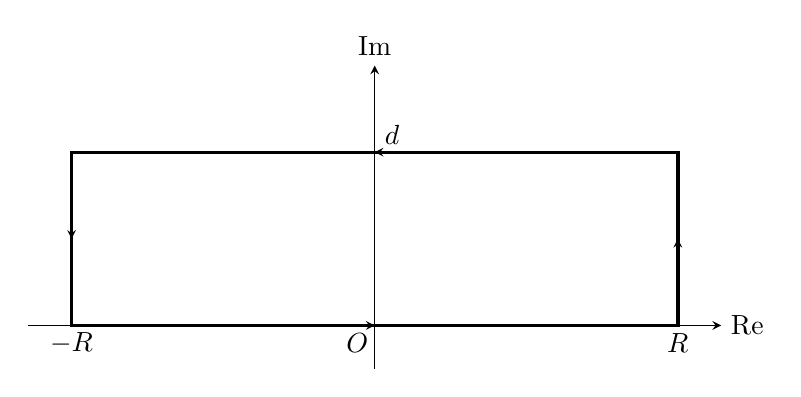
\begin{tikzpicture}[>=stealth,scale=1.1]
            \draw[->](-4,0)--(4,0) node[right] {Re};
            \draw[->](0,-0.5)--(0,3) node[above] {Im};
            \draw[very thick] (-3.5,0)--(3.5,0)--(3.5,2)--(-3.5,2)--cycle;
            \draw[->] (-0.2,0)--(0,0);
            \draw[->] (0.2,2)--(0,2);
            \draw[->] (3.5,0.8)--(3.5,1);
            \draw[->] (-3.5,1.2)--(-3.5,1);
            \node at(-3.5,-0.2) {$-R$};
            \node at(3.5,-0.2) {$R$};
            \node at(0.2,2.2) {$\imag d$};
            \node at(-0.2,-0.2) {$O$};
        \end{tikzpicture}
    \end{center}
    $e^{-az^{2}}$に留数は存在しないので, 上の周回積分路$C$において
    \begin{eqnarray*}
        \dint[z]{C}{}{\exp(-az^{2})}=0 
    \end{eqnarray*}
    ここで, $-R\to R$の積分路を$C_{1}$とし, $R\to R+\imag d$の積分路を$C_{2}$, $R+\imag d\to -R+\imag d$の積分路を$C_{3}$, $-R+\imag d\to -R$の積分路を$C_{4}$とすると,
    \begin{eqnarray*}
        C = C_{1}+C_{2}+C_{3}+C_{4}
    \end{eqnarray*}
    である. ここで,$R \to \infty$において
    \begin{eqnarray*}
        \lim_{R\to \infty}\dint[z]{C_{2}}{}{\exp(-az^{2})} 
        &=& \lim_{R\to \infty}\dint[t]{0}{d}{\exp(-a(R+\imag t)^{2})}\\
        &=&0
    \end{eqnarray*}
    同様にして
    \begin{eqnarray*}
        \lim_{R\to \infty}\dint[z]{C_{4}}{}{\exp(-az^{2})} 
        &=& \lim_{R\to \infty}\dint[t]{d}{0}{\exp(-a(-R+\imag t)^{2})}\\
        &=& 0
    \end{eqnarray*}
    となるので,
    \begin{eqnarray*}
        \lim_{R\to \infty}\dint[z]{C}{}{\exp(-az^{2})} 
        &=& \lim_{R\to \infty}\dint[z]{C_{1}}{}{\exp(-az^{2})}+\lim_{R\to \infty}\dint[z]{C_{3}}{}{\exp(-az+\imag d)}\\
        &=& 0
    \end{eqnarray*}
    したがって,
    \begin{eqnarray*}
        \dint{-\infty}{\infty}{\exp(-ax^{2})} = \dint{-\infty}{\infty}{\exp(-a(x+\imag d)^{2})}
    \end{eqnarray*}
    ここで, $t=\sqrt{a}x$とおくと,
    \begin{eqnarray*}
        \frac{{\rm d}t}{{\rm d}x}=\sqrt{a}\ \Longleftrightarrow\ {\rm d}x = \frac{1}{\sqrt{a}}\,{\rm d}t
    \end{eqnarray*}
    であるから,
    \begin{eqnarray*}
        \dint{-\infty}{\infty}{\exp(-ax^{2})} &=& \dint[t]{-\infty}{\infty}{\exp(-t^{2})\cdot \frac{1}{\sqrt{a}}}\\
                                              &=& \frac{1}{\sqrt{a}}\dint{-\infty}{\infty}{\exp(-x^{2})}\\
                                              &=& \sqrt{\frac{\pi}{a}}
    \end{eqnarray*}
    よって,
    \begin{eqnarray*}
        \dint{-\infty}{\infty}{\exp(-a(x+\imag d))} = \sqrt{\frac{\pi}{a}}
    \end{eqnarray*}
    \item 
    \begin{enumerate}[(i)]
        \setlength{\itemsep}{10pt}
        \item 式\eqref{eq:subsec2:prom2}と題意より,以下が成り立つ.
        \begin{align*}
            \pdiff[2]{U(k, t)}{t} 
            & = \pdiff[2]{\left(\frac{1}{\sqrt{2\pi}}\dint{-\infty}{\infty}{u(x, t)\exp(-\imag kx)}\right)}{t}\\
            & = \frac{1}{\sqrt{2\pi}}\dint{-\infty}{\infty}{\pdiff[2]{u(x, t)}{t}\exp(-\imag kx)}\\
            & = \frac{1}{\sqrt{2\pi}}\dint{-\infty}{\infty}{c^{2}\pdiff[2]{u(x, t)}{x}\exp(-\imag kx)}\\
            & = \frac{c^{2}}{\sqrt{2\pi}}\left\{\left[\pdiff{u(x, t)}{x}\exp(-\imag kx)\right]_{-\infty}^{\infty} - (-\imag k)\dint{-\infty}{\infty}{\pdiff{u(x, t)}{x}\exp(-\imag kx)}\right\}\\
            & = \frac{\imag kc^{2}}{\sqrt{2\pi}}\dint{-\infty}{\infty}{\pdiff{u(x, t)}{x}\exp(-\imag kx)}\\
            & = \frac{\imag kc^{2}}{\sqrt{2\pi}}\left\{\left[u(x, t)\exp(-\imag kx)\right]_{-\infty}^{\infty} - (-\imag k)\dint{-\infty}{\infty}{u(x, t)\exp(-\imag kx)}\right\}\\
            & = \frac{(\imag kc)^{2}}{\sqrt{2\pi}}\dint{-\infty}{\infty}{u(x, t)\exp(-\imag kx)}\\
            & = -(kc)^{2}U(k, t)
        \end{align*}
        よって,$U(k, t)$は以下の偏微分方程式に従う.
        \begin{equation}
            \pdiff[2]{U(k, t)}{t} = -(kc)^{2}U(k, t)\label{eq:subsec2:ans1}
        \end{equation}
        \item 初期条件\eqref{eq:subsec2:prom2_syoki2}より,以下のことが成り立つ.
        \begin{align*}
            \pdiff{U(k, t)}{t} 
            & = \pdiff{\left(\frac{1}{\sqrt{2\pi}}\dint{-\infty}{\infty}{u(x, t)\exp(-\imag kx)}\right)}{t}\\
            & = \frac{1}{\sqrt{2\pi}}\dint{-\infty}{\infty}{\pdiff{u(x, t)}{t}\exp(-\imag kx)}\\
        \end{align*}
        \begin{equation}
            \therefore\, \pdiff{U}{t}(k, 0) 
             = \frac{1}{\sqrt{2\pi}}\dint{-\infty}{\infty}{\pdiff{u}{t}(x, 0)\exp(-\imag kx)} = 0\label{eq:subsec2:ans2_ini1}
        \end{equation}
        よって,$U(k, t)$に関する初期条件も式\eqref{eq:subsec2:ans2_ini1}のようになる.ここで$U(k, t)$が題意の関数で表されるとすると
        $U(k, t)$の$t$に関する1階偏微分を行うと以下のようになる.
        \begin{align*}
            \pdiff{U(k, t)}{t} &= \pdiff{F(k)\cos(kct)}{t}\\
            &= F(k)(-kc\sin(kct))
        \end{align*}
        よって,以下が成り立つ.
        \begin{equation}
            \pdiff{U}{t}(k, 0) = F(k)(-kc\sin(kc\cdot 0)) = 0\label{eq:subsec2:ans2_ini2}
        \end{equation}
        よって,題意の関数でおくと初期条件\eqref{eq:subsec2:ans2_ini1}を満たす.
        また,\eqref{subsec2:prom2:prom1}の解となるかを以下に示す.
        
        \eqref{subsec2:prom2:prom1}の式に代入して,
        \begin{align*}
            \mbox{(左辺)}
            &= \pdiff[2]{U(k, t)}{t} \\
            &= \pdiff[2]{\left(F(k)\cos(kct)\right)}{t}\\
            &= -(kc)^{2}F(k)\cos(kct)\\
            &= -(kc)^{2}U(k, t)\\
            &= \mbox{(右辺)}
        \end{align*}
        よって,$U(k, t) = F(k)\cos(kct)$は\eqref{subsec2:prom2:prom1}の解の一つである.従って,式\eqref{eq:subsec2:prom2_syoki2}
        の初期条件のもとで\eqref{subsec2:prom2:prom1}の解となることが示されたので,題意は示された.
        \item 式\eqref{eq:subsec2:prom2_syoki1}の初期条件の下で設問\eqref{subsec2:prom1}より,以下が成り立つ.
        \begin{align*}
            U(k, 0) &= \frac{1}{\sqrt{2\pi}}\dint{-\infty}{\infty}{u(x, 0)\exp(-\imag kx)}\\ 
            &= \frac{1}{\sqrt{2\pi}}\dint{-\infty}{\infty}{\exp\left(-ax^{2}\right)\exp(-\imag kx)}\\
            &= \frac{1}{\sqrt{2\pi}}\dint{-\infty}{\infty}{\exp\left(-ax^{2}-\imag kx\right)}\\
            &= \frac{1}{\sqrt{2\pi}}\dint{-\infty}{\infty}{\exp\left\{-a\left(x - \frac{\imag k}{2a}\right)^{2} + \frac{1}{a}\cdot \left(\frac{\imag k}{2}\right)^{2}\right\}}\\
            &= \frac{\exp \left(-\frac{k^{2}}{4a}\right)}{\sqrt{2\pi}}\dint{-\infty}{\infty}{\exp\left\{-a\left(x - \frac{\imag k}{2}\right)^{2}\right\}}\\
            &= \frac{\exp \left(-\frac{k^{2}}{4a}\right)}{\sqrt{2\pi}}\sqrt{\frac{\pi}{a}}
        \end{align*}
        従って以下が成り立つ.
        \begin{align*}
            U(k, 0) = F(k)\cos(kc\cdot 0) = F(k) = \frac{\exp \left(-\frac{k^{2}}{4a}\right)}{\sqrt{2a}}
        \end{align*}
        よって,$U(k, t)$は以下のようになる
        \begin{equation}
            U(k, t) = F(k)\cos(kct) = \frac{\exp \left(-\frac{k^{2}}{4a}\right)}{\sqrt{2a}}\cos(kct)
        \end{equation}
    \end{enumerate}
  \item 設問\eqref{subsec2:prom2}で得られた$U(k, t)$と$a > 0$, 設問\eqref{subsec2:prom1}より,以下が成り立つ.
    \begin{align*}
        u(x, t) &= \frac{1}{\sqrt{2\pi}}\dint[k]{-\infty}{\infty}{U(k, t)\exp(ikx)}\\
        &= \frac{1}{\sqrt{2\pi}}\dint[k]{-\infty}{\infty}{\frac{\exp\left(\frac{-ak^2}{4}\right)}{\sqrt{2a}}\cos(kct)\exp(\imag kx)}\\
        &= \frac{1}{2\sqrt{a\pi}}\dint[k]{-\infty}{\infty}{\exp\left(-a\frac{k^2}{4} + \imag kx\right)\frac{\exp\left(\imag kct\right) + \exp\left(-\imag kct\right)}{2}}\\
        &= \frac{1}{4\sqrt{a\pi}}\dint[k]{-\infty}{\infty}{\exp\left(-a\frac{k^2}{4} + \imag kx + \imag kct\right) + \exp\left(-a\frac{k^2}{4} + \imag kx - \imag kct\right)}\\
        &= \frac{1}{4\sqrt{a\pi}}\dint[k]{-\infty}{\infty}{\exp\left\{-\frac{a}{4}\left(k - 2\imag \frac{x + ct}{a}\right)^2 + \frac{(x + ct)^2}{a}\right\}}\\
        &\quad+ \frac{1}{4\sqrt{a\pi}}\dint[k]{-\infty}{\infty}{\exp\left\{-\frac{a}{4}\left(k - 2\imag \frac{x - ct}{a}\right)^2 + \frac{(x - ct)^2}{a}\right\}}\\
        &= \frac{1}{4\sqrt{a\pi}}\exp\left\{\frac{(x + ct)^2}{a}\right\}\dint[k]{-\infty}{\infty}{\exp\left\{-\frac{a}{4}\left(k - 2\imag \frac{x + ct}{a}\right)^2\right\}}\\
        &\quad+ \frac{1}{4\sqrt{a\pi}}\exp\left\{\frac{(x - ct)^2}{a}\right\}\dint[k]{-\infty}{\infty}{\exp\left\{-\frac{a}{4}\left(k - 2\imag \frac{x - ct}{a}\right)^2\right\}}\\
        &= \frac{1}{4\sqrt{a\pi}}\exp\left\{\frac{(x + ct)^2}{a}\right\}\sqrt{\frac{\pi}{\frac{a}{4}}} + \frac{1}{4\sqrt{a\pi}}\exp\left\{\frac{(x - ct)^2}{a}\right\}\sqrt{\frac{\pi}{\frac{a}{4}}}\\
        &= \frac{1}{2a}\left[\exp\left\{\frac{(x + ct)^2}{a}\right\} + \exp\left\{\frac{(x - ct)^2}{a}\right\}\right]
    \end{align*}
    よって,求める関数$u(x, t)$は以下のようになる.
    \begin{equation*}
        u(x, t) = \frac{1}{2a}\left[\exp\left\{\frac{(x + ct)^2}{a}\right\} + \exp\left\{\frac{(x - ct)^2}{a}\right\}\right]
    \end{equation*}
\end{enumerate}

\newpage

\section{}%第3問
\subsection{問題文}
下図のように,平面上に三角形$\mathrm{ABC}$が与えられており,各頂点の座標は
$\mathrm{A(1, 0), B(0, 1), C(-1, -1)}$とする.原点$(0, 0)$を端点とする半直線$\ell$をランダムに選ぶ.
すなわち,$\Theta$を区間$[0, 2\pi)$上の一様分布に従う確率変数として,
\begin{equation*}
    \ell = \left\{(r\cos\Theta, r\sin\Theta) \mid r \geq 0\right\}
\end{equation*}
とおく.この半直線$\ell$と三角形$\mathrm{ABC}$の周との交点を$\mathrm{Q}$とおく.また,$\mathrm{Q}$の座標を
$(X, Y)$とおく.ただし,$X, Y$は確率変数である.以下の問いに答えよ.
\begin{enumerate}[(1)]
    \setlength{\itemsep}{10pt}
    \item 点$\mathrm{Q}$が辺$\mathrm{AB}$上にある確率を求めよ.\label{subsec3:prom1}
    \item 点$\mathrm{Q}$が辺$\mathrm{AB}$上にあるという条件の下での$X$の期待値は$1/2$であることを示せ.但し,
    三角形$\mathrm{ABC}$が直線$y = x$に関して対称であることを利用してもよい.\label{subsec3:prom2}
    \item 点$\mathrm{Q}$が辺$\mathrm{BC}$にあるという条件のもとでの$X$の確率密度関数を,変数変換の公式
    \begin{equation*}
        f(x) = g(h(x))\left\lvert \diff{h}{x}(x) \right\rvert
    \end{equation*}
    を使って求めよ.ただし,$x$は任意の実数とし,$f$と$g$はそれぞれ$X$と$\Theta$の確率密度関数を表し,$h$は$\Theta = h(X)$を満たす関数とする.\label{subsec3:prom3}
    \item 点$\mathrm{Q}$が辺$\mathrm{BC}$にあるという条件のもとでの$X$の期待値を$\alpha$とおく.設問\ref{subsec3:prom3}の結果を用いて$\alpha$
    を求めよ.\label{subsec3:prom4}
    \item $X$の期待値$\mu$を求めよ.
\end{enumerate}
\begin{figure}[htbp]
    \centering
    \begin{tikzpicture}[>=stealth, scale = 1.5]
        \coordinate (O) at (0, 0) node at (O) [below left] {$\mathrm{O}$};
        \coordinate (A) at (2, 0) node at (A) [below] {$\mathrm{A(1, 0)}$};
        \coordinate (B) at (0, 2) node at (B) [right] {$\mathrm{B(0, 1)}$};
        \coordinate (C) at (-2, -2) node at (C) [below] {$\mathrm{C(-1, -1)}$};
        \draw (A) -- (B) -- (C) -- cycle;
        \draw [name path = AB] (A) -- (B);
        \draw [->] ($(O) + (-2.8, 0)$) -- ($(O) + (2.8, 0)$);%x軸
        \draw [->] ($(O) + (0, -2.8)$) -- ($(O) + (0, 2.8)$);%y軸
        \draw [domain = 0:2.5, name path = l] plot(\x, 1/2*\x) node [above] {$\ell$};
        \draw [fill = black, name intersections = {of = l and AB}]
		(intersection-1) circle [radius = 0.5mm] node [right = 0.2cm] {$\mathrm{Q}(X, Y)$};
    \end{tikzpicture}
\end{figure}

\newpage

\subsection{解答例}
\begin{enumerate}[(1)]
  \setlength{\itemsep}{10pt}
\item 点$\mathrm{Q}$が辺$\mathrm{AB}$にある時,確率変数$\Theta$は以下の範囲に存在する.
  \begin{equation}
    0\, \leq\, \Theta\, \leq\, \frac{\pi}{2}\label{eq:subsec3:prom1:hanni}
  \end{equation}
  ここで,確率変数$\Theta$は区間$[0, 2\pi)$上の一様分布に従う確率変数であるので,
  $\Theta$に関する確率密度関数$f_{\Theta}(\Theta)$は定数$c\, \in \mathbb{R}$を用いて,以下のように定義される.
  \begin{align}
    f_{\Theta}(\Theta) = 
    \begin{cases}
      c & 0\, \leq\, \Theta\, <\, 2\pi\\
      0 & 0 > \Theta,\, \Theta\, \geq\, 2\pi
    \end{cases} \label{eq:subsec3:prom1:ftheta}
  \end{align}
  よって,式\eqref{eq:subsec3:prom1:ftheta}と確率密度関数の定義より,以下が成り立つ.
  \begin{align*}
    \dint[\Theta]{-\infty}{\infty}{f_{\Theta}(\Theta)} = 1\\
    \Longleftrightarrow\; &\lim_{x \to 2\pi-0}\dint[\Theta]{0}{x}{c} = 1\\
    \Longleftrightarrow\; &\lim_{x \to 2\pi-0}cx = 1\\
    \Longleftrightarrow\; &2c\pi = 1\\
    \Longleftrightarrow\; &c = \frac{1}{2\pi}
  \end{align*}
  よって,式\eqref{eq:subsec3:prom1:ftheta}から$f_{\Theta}(\Theta)$は以下のように定義し直すことができる.
  \begin{align}
    f_{\Theta}(\Theta) = 
    \begin{cases}
      \frac{1}{2\pi} & 0\, \leq\, \Theta\, <\, 2\pi\\
      0 & 0 > \Theta,\, \Theta\, \geq\, 2\pi
    \end{cases}\label{eq:subsec3:prom1:f}
  \end{align}
  従って式\eqref{eq:subsec3:prom1:f}, \eqref{eq:subsec3:prom1:hanni}から求める確率$P$は以下のようになる.
  \begin{align*}
    P &= \dint[\Theta]{0}{\cfrac{\pi}{2}}{f_{\Theta}(\Theta)} = \dint[\Theta]{0}{\cfrac{\pi}{2}}{\frac{1}{2\pi}}\\
      &= \frac{1}{2\pi}\frac{\pi}{2} = \frac{1}{4}
  \end{align*}
  よって,求める確率は$\frac{1}{4}$になる.\\[1cm]
  (中田解)\\
  QがAB上にある確率とは, Qが第1象限上に存在する確率と等しい. ここで, $\Theta$は区間$[0,2\pi)$上の一様分布に従う確率変数であるので, 半直線$l$が第1象限上に存在する確率は$\displaystyle \frac{1}{4}$である. よって答えは$\displaystyle \frac{1}{4}$である.
\item 設問\eqref{subsec3:prom1}より,辺$\mathrm{AB}$上に点$\mathrm{Q}$が存在するときは$0\, \leq \, \Theta\, \leq \frac{\pi}{2}$を満たす.
  
  また,この時,題意より確率変数$X$について以下が成り立つ.
  
  $\ell$の方程式: 
  \begin{align}
    X = r\cos\Theta, \, Y = r\sin\Theta\, 
    \therefore X\sin\Theta = Y\cos\Theta\label{eq:subsec3:prom2:prex}\\
  \end{align}
  辺$\mathrm{AB}$の方程式:
  \begin{equation*}
    (y - 1) = \frac{0 - 1}{1 - 0}(x - 0)\, \therefore y = -x + 1\, (0\, \leq \, x \, \leq \, 1)
  \end{equation*}
  よって点$\mathrm{Q}$が$\mathrm{AB}$上にあるので
  \begin{equation}
    Y = -X + 1\, (0\, \leq\,  X\, \leq \, 1)\label{eq:subsec3:prom2:tyokkou}\\
  \end{equation}
  式\eqref{eq:subsec3:prom2:prex}, \eqref{eq:subsec3:prom2:tyokkou}より$0\, \leq\, X\, \leq\, 1$において
  \begin{align}
    X\sin\Theta &= (-X + 1)\cos\Theta\nonumber\\
    \therefore \cos\Theta &= X(\sin\Theta + \cos\Theta)\label{eq:subsec3:prom2:inix}
  \end{align}
  ここで$\sin\Theta + \cos\Theta = \sqrt{2}\sin\left(\Theta + \frac{\pi}{4}\right)$であるため,
  $0\, \leq\, \Theta\, \leq \, \frac{\pi}{2}$における範囲は以下のようになる.
  \begin{align}
    \sqrt{2}\times\frac{1}{\sqrt{2}} \leq\, &\sqrt{2}\sin\left(\Theta + \frac{\pi}{4}\right) \, \leq\, \sqrt{2}\nonumber\\
    \Longleftrightarrow 
    1 \leq\, &\sin\Theta + \cos\Theta \, \leq\, \sqrt{2}\label{eq:subsec3:prom2:hanni}
  \end{align}
  よって,式\eqref{eq:subsec3:prom2:inix}, \eqref{eq:subsec3:prom2:hanni}より,$X$は以下のように表せる.
  \begin{equation}
    X = \frac{\cos\Theta}{\sin\Theta + \cos\Theta} = \frac{\cos\Theta}{\sqrt{2}\sin\left(\Theta + \frac{\pi}{4}\right)}\label{eq:subsec3:prom2:x}
  \end{equation}
  ここで$0\, \leq\, \Theta\, \leq\, \frac{\pi}{2}$において,
  $X$を$\Theta$の関数$F(\Theta)$として考えると以下が成り立つ.
  \begin{align*}
    \diff{F}{\Theta}(\Theta) 
    &= \frac{-\cos\left\{\Theta - \left(\Theta + \frac{\pi}{4}\right)\right\}}{\sqrt{2}\sin^{2}\left(\Theta + \frac{\pi}{4}\right)}\\
    &= -\frac{1}{2\sin^{2}\left(\Theta + \frac{\pi}{4}\right)} < 0
  \end{align*}
  よって,$0\, \leq\, \Theta\, \leq\, \frac{\pi}{2}$において,$X = F(\Theta)$は単調減少することが分かる.
  従って,$0\, \leq\, \Theta\, \leq\, \frac{\pi}{2}$において,ある$\Theta$に対応する$X$の値はただ一つしか存在
  しないので,$X$も$0\, \leq\, X\, \leq\, 1$において一様分布に従う.よって,この区間における確率密度関数$f_{X_{01}}(X)$は以下のようになる.
  \begin{align*}
    f_{X_{01}}(X) = 
    \begin{cases}
      c_{X} & 0\, \leq\, X\, \leq\, 1\\
      0 & X < 0, \, X > 1    
    \end{cases}
  \end{align*}
  よって,確率密度関数の性質より
  \begin{align*}
    \dint[X]{-\infty}{\infty}{f_{X_{01}}(X)} &= 1\\
    \dint[X]{0}{1}{f_{X_{01}}(X)} &= 1\\
    \dint[X]{0}{1}{c_{X}} &= 1\\
    c_{X} = 1
  \end{align*}
  従って,点$\mathrm{Q}$が辺$\mathrm{AB}$上にある条件の下での$X$の期待値$E_{X}$は以下のようになる.
  \begin{align*}
    E_{X} &= \dint[X]{-\infty}{\infty}{Xf_{X_{01}}(X)}\\
          &= \dint[X]{0}{1}{X}\\
          &= \frac{1}{2}
  \end{align*}
  よって,題意は示された.\\[1cm]
  (中田解)\\
  三角形ABCが直線$y=x$に関して対称であることから一様分布に従う確率変数のもとでは期待値は$y=x$上に存在する. ここで, 点Qが辺AB上にあるという条件下においては辺ABと$y=x$の交点が期待値であることがいえる. ここで交点を求めると$\displaystyle \left(\frac{1}{2},\frac{1}{2}\right)$であるから求める$X$の期待値は1/2である. よって, 題意は示された.
\item 以降$\arctan x$の定義域は$-\frac{\pi}{2} < x < \frac{\pi}{2}$であるとする.
  
  点$\mathrm{Q}$が辺$\mathrm{BC}$上にあるので,確率変数$X$に関して以下が成り立つ.
    
  辺$\mathrm{BC}$の方程式:
  \begin{equation*}
    (y - 1) = \frac{1 + 1}{0 + 1}(x - 0)\, \therefore y = 2x + 1
  \end{equation*}
  よって点$\mathrm{Q}$が$\mathrm{BC}$上にあるので$-1\, \leq\, X\, \leq\, 0$において
  \begin{equation}
    Y = 2X + 1\label{eq:subsec3:prom3:tyokkou}
  \end{equation}
  点$\mathrm{Q}$は半直線$\ell$上の点でもあるので,式\eqref{eq:subsec3:prom2:prex}, \eqref{eq:subsec3:prom3:tyokkou}より$-1\, \leq\, X\, \leq\, 0$において
  \begin{align}
    X\sin\Theta &= \left(2X + 1\right)\cos\Theta\nonumber\\
                &\therefore
                  \begin{cases}
                    \Theta = \frac{\pi}{2} & X = 0\\
                    \sin\Theta = \frac{2X + 1}{X}\cos\Theta & -1\, \leq\, X < 0
                  \end{cases}\label{eq:subsec3:prom3:theta1}
  \end{align}
  よって,$X \neq 0$の時$\Theta \neq \frac{\pi}{2}$であるので$\cos\Theta \neq 0$
  であり,式\eqref{eq:subsec3:prom3:theta1}より$\Theta$について点$\mathrm{Q}$が辺$\mathrm{BC}$に
  存在する場合,$\frac{\pi}{2} \, \leq\, \Theta\, \leq\, \frac{5\pi}{4}$より以下が成り立つ.
  \begin{align}
    &\begin{cases}
      \Theta = \frac{\pi}{2} & X = 0\\
      \tan\Theta = \frac{2X + 1}{X} & -1\, \leq\, X < 0\\
    \end{cases}\nonumber\\
    \Longleftrightarrow&
                         \begin{cases}
                           \Theta = \frac{\pi}{2} & X = 0\\
                           \Theta = \pi + \arctan\left(\frac{2X + 1}{X}\right) & -1\, \leq\, X < 0\\
                         \end{cases}\label{eq:subsec3:prom3:theta2}
  \end{align}
  $\Theta$は区間$[0, 2\pi)$において一様分布に従うので確率密度関数$g(\Theta)$は式
  \eqref{eq:subsec3:prom1:f}であるため,以下が成り立つ.
  \begin{equation*}
    g(\Theta) = \frac{1}{2\pi}
  \end{equation*}
  $\frac{\pi}{2} < \Theta \leq \frac{5\pi}{4}$において,つまり$ -1\, \leq\, X < 0$の時,
  式\eqref{eq:subsec3:prom3:theta2}より確率密度関数$f(x)$は変数変換の公式を用いて以下のようになる
  \begin{align}
    \Theta = h(X) &= \pi + \arctan\left(\frac{2X + 1}{X}\right) \nonumber\\
    \therefore \diff{h}{x}(x) &= \frac{1}{1 + \left(\frac{2x + 1}{x}\right)^2}\frac{2x - (2x + 1)}{x^2}\nonumber\\
                  &= \frac{-x^2}{\left\{\left(2x + 1\right)^2 + x^2\right\}x^2}\nonumber\\
                  &= \frac{-1}{\left(2x + 1\right)^2 + x^2}\nonumber\\
    \Longleftrightarrow 
    f(x) &= \frac{1}{2\pi}\frac{-1}{\left(2x + 1\right)^2 + x^2}\label{eq:subsec3:prom3:fx:nez}
  \end{align}
  $\Theta = \frac{\pi}{2}$において,つまり$X = 0$の時,
  式\eqref{eq:subsec3:prom3:theta2}より確率密度関数$f(x)$は変数変換の公式を用いて以下のようになる
  \begin{align}
    \Theta = h(0) &= \frac{\pi}{2}\nonumber\\
    \diff{h}{x} &= 0\nonumber\\
    \Longleftrightarrow f(0) &= 0\label{eq:subsec3:prom3:fx:ez}
  \end{align}
  よって,式\eqref{eq:subsec3:prom3:fx:nez},\eqref{eq:subsec3:prom3:fx:ez}より, 求める確率密度関数$f(x)$は以下のようになる.
  \begin{equation*}
    f(x) = 
    \begin{cases}
      0 & x = 0\\
      \frac{-1}{2\pi\left\{\left(2x + 1\right)^2 + x^2\right\}} & -1\, \leq\, x < 0
    \end{cases}
  \end{equation*}
  \vspace{0.7cm}
  
  \noindent (中田解)\\
  辺BC上を通る直線の式は$y=2x+1$である. ここで辺BC上に点Qが存在する確率密度関数は$\Theta$の範囲が$\displaystyle \left[\frac{\pi}{2},\frac{5}{4}\pi\right]$であるから,
  \begin{eqnarray*}
    g(x) = \frac{4}{3\pi}
  \end{eqnarray*}
  $X,\ \Theta$の関係について$Y=2X+1$であることと, $X=r\cos \Theta,\ Y=r\sin \Theta$であることから,
  \begin{eqnarray*}
    \tan \Theta X = 2X+1
  \end{eqnarray*}
  となる. $X=0$のとき, $\displaystyle \Theta=\frac{\pi}{2}$である. $X\neq 0$のときは
  \begin{eqnarray*}
    &&\tan \Theta X = 2X+1\\
    \Longleftrightarrow\ &&\tan \Theta = 2+\frac{1}{X}\\
    \Longleftrightarrow\ &&\Theta = {\rm Arctan} \left(2+\frac{1}{X}\right)
  \end{eqnarray*}
  ゆえに
  \begin{eqnarray*}
    h(X) = {\rm Arctan} \left(2+\frac{1}{X}\right)
  \end{eqnarray*}
  よって,
  \begin{eqnarray*}
    f(x) &=& g(h(x))\left|\frac{{\rm d}h}{{\rm d}x}(x)\right|\\
         &=& \frac{4}{3\pi}\left|\frac{1}{1+\left(2+\frac{1}{x}\right)^{2}}\cdot \left(-\frac{1}{x^{2}}\right)\right|\\
         &=& \left|\frac{4}{3\pi}\cdot \frac{1}{5x^{2}+4x+1}\right|\\
         &=& -\frac{4}{3\pi}\cdot \frac{1}{5x^{2}+4x+1}
  \end{eqnarray*}
  $x=0$に関しても連続であるから同様の答えとなる. 
\item 設問\eqref{subsec3:prom3}より辺$\mathrm{BC}$上に点$\mathrm{Q}$
  が存在する時の$X$の期待値$\alpha$は以下のようになる.
  \begin{align*}
    \alpha &= \dint{-\infty}{\infty}{xf(x)}\\
           &= \lim_{t \to -0}\dint{-1}{t}{xf(x)}\\
           &= \lim_{t \to -0}\dint{-1}{t}{\frac{-x}{2\pi\left\{\left(2x + 1\right)^2 + x^2\right\}}}\\
           &= \lim_{t \to -0}\frac{-1}{20\pi}\dint{-1}{t}{\frac{10x + 4 - 4}{\left(2x + 1\right)^2 + x^2}}\\
           &= \lim_{t \to -0}\frac{-1}{20\pi}\left\{\left[\log\left\{\left(2x + 1\right)^2 + x^2\right\}\right]_{-1}^{t} - \dint{-1}{t}{\frac{4}{\left(2x + 1\right)^2 + x^2}}\right\}\\
           &= \lim_{t \to -0}\left(\frac{-1}{20\pi}\left[\log\left\{\left(2t + 1\right)^2 + t^2\right\} - \log 2\right] + \frac{1}{5\pi}\dint{-1}{t}{\frac{1}{\frac{1}{5}\left\{\left(5x + 2\right)^2 + 1\right\}}}\right)\\
           &= \frac{\log 2}{20\pi} + \lim_{t \to -0}\frac{1}{\pi}\dint{-1}{t}{\frac{1}{\left(5x + 2\right)^2 + 1}}
  \end{align*}
  ここで$5x + 2 = \tan u$と置換し, $\beta, \gamma$を$\tan\beta = -3, \tan\gamma = 5t + 2$を満たすとものとしておくと以下のようになる.
  \begin{align*}
    \alpha &= \frac{\log 2}{20\pi} + \lim_{t \to -0}\frac{1}{\pi}\dint[u]{\beta}{\gamma}{\frac{1}{\tan^{2}u+ 1}\frac{1}{5\cos^{2}u}}\\
           &= \frac{\log 2}{20\pi} + \lim_{t \to -0}\frac{1}{5\pi}(\gamma - \beta)\\
           &= \frac{\log 2}{20\pi} + \lim_{t \to -0}\frac{1}{5\pi}\bigl\{(\pi + \arctan(5t + 2)) - (\pi + \arctan(-3))\bigr\}\\
           &= \frac{\log 2}{20\pi} + \frac{1}{5\pi}(\arctan 2 + \arctan 3)
  \end{align*}
  よって,期待値$\alpha$について以下のようになる.
  \begin{equation}
    \alpha = \frac{\log 2}{20\pi} + \frac{1}{5\pi}(\arctan 2 + \arctan 3)\label{eq:subsec3:prom4:ans}
  \end{equation}
  \vspace{0.3cm}

  \noindent (中田解)\\
  (3)の結果を用いて以下のように期待値は表せる.
  \begin{eqnarray*}
    \alpha &=& \int_{-1}^{0}xf(x)\ {\rm d}x\\
           &=& \int_{-1}^{0}\left(-\frac{4}{3\pi}\cdot\frac{1}{5x^{2}+4x+1}\right)\cdot x\ {\rm d}x\\
           &=& -\frac{4}{3\pi}\int_{-1}^{0}\frac{x}{5x^{2}+4x+1}\ {\rm d}x\\
           &=& -\frac{4}{3\pi}\int_{-1}^{0}\frac{1}{10}\left(\frac{10x+4}{5x^{2}+4x+1}-\frac{4}{5x^{2}+4x+1}\right)\ {\rm d}x\\
           &=& -\frac{2}{15\pi}\left(\Bigl[\log\left|5x^{2}+4x+1\right|\Bigr]_{-1}^{0}-4\int_{-1}^{0}\frac{1}{5x^{2}+4x+1}\ {\rm d}x\right)\\
           &=& -\frac{2}{15\pi}\left(-\log 2-4\int_{-1}^{0}\frac{1}{5\left(x^{2}+\frac{4}{5}x\right)+1}\ {\rm d}x\right)\\
           &=& -\frac{2}{15\pi}\left(-\log 2-4\int_{-1}^{0}\frac{1}{5\left\{\left(x+\frac{2}{5}\right)^{2}-\frac{4}{25}\right\}+1}\ {\rm d}x\right)\\
           &=& -\frac{2}{15\pi}\left(-\log 2-4\int_{-1}^{0}\frac{1}{5\left(x+\frac{2}{5}\right)^{2}+\frac{1}{5}}\ {\rm d}x\right)\\
           &=& -\frac{2}{15\pi}\left(-\log 2-4\int_{-1}^{0}5\cdot \frac{1}{25\left(x+\frac{2}{5}\right)^{2}+1}\ {\rm d}x\right)\\
           &=& -\frac{2}{15\pi}\left(-\log 2-\left[4\cdot 5\cdot \frac{1}{5}\cdot {\rm Arctan} \left\{5\cdot \left(x+\frac{2}{5}\right)\right\}\right]_{-1}^{1}\right)\\
           &=&-\frac{2}{15\pi}\Bigl\{-\log 2-4\cdot \left({\rm Arctan}2+{\rm Arctan 3}\right)\Bigr\}\\
           &=&-\frac{2}{15\pi}\left\{-\log 2-4\cdot \left(-\frac{\pi}{4}\right)\right\}\\
           &=& \frac{2}{15\pi}\log 2-\frac{2}{15}
  \end{eqnarray*}
\item まず,点$\mathrm{Q}$が辺$\mathrm{AC}$上にある時の$X$の期待値$\delta$を求める.
  
  設問\eqref{subsec3:prom4}, \eqref{subsec3:prom3}と同様にして確率密度関数を求めてから期待値を求める.
  
  この時,確率変数$X$について以下のことが成り立つ.
  
  辺$\mathrm{AC}$の方程式:
  \begin{equation*}
    (y - 0) = \frac{0 + 1}{1 + 1}(x - 1)\, \therefore y = \frac{1}{2}(x - 1)
  \end{equation*}
  よって点$\mathrm{Q}$が$\mathrm{AC}$上にあるので$-1\, \leq\,  X\, \leq \, 1$において
  \begin{equation}
    Y = \frac{1}{2}(X - 1)\label{eq:subsec3:prom4:tyokkou}
  \end{equation}
  点$\mathrm{Q}$は半直線$\ell$上の点でもあるので,式\eqref{eq:subsec3:prom2:prex}, 
  \eqref{eq:subsec3:prom4:tyokkou}より$-1\, \leq\,  X\, \leq \, 1$において
  \begin{align}
    X\sin\Theta &= \frac{1}{2}\left(X - 1\right)\cos\Theta\nonumber\\
                &\therefore
                  \begin{cases}
                    \Theta = \frac{3\pi}{2} & X = 0\\
                    \sin\Theta = \frac{X - 1}{2X}\cos\Theta & -1\, \leq\, X < 0,\, 0 < X\, \leq\, 1
        \end{cases}\label{eq:subsec3:prom4:theta1}
  \end{align}
  よって,$X \neq 0$の時$\Theta \neq \frac{3\pi}{2}$であるので$\cos\Theta \neq 0$であり,
  式\eqref{eq:subsec3:prom4:theta1}より$\Theta$について点$\mathrm{Q}$が辺$\mathrm{AC}$
  に存在する場合,つまり,$-1\, \leq\, X\, \leq\, 1$において以下が成り立つ.
  \begin{align}
    &\begin{cases}
      \Theta = \frac{3\pi}{2} & X = 0\\
      \tan\Theta = \frac{X - 1}{2X} & -1\, \leq\, X < 0,\, 0 < X\, \leq\, 1\\
    \end{cases}\nonumber\\
    \Longleftrightarrow&
                         \begin{cases}
                           \Theta = \frac{3\pi}{2} & X = 0\\
                           \Theta = \pi + \arctan\left(\frac{X - 1}{2X}\right) & 0 < X \, \leq\, 1\\
                           \Theta = 2\pi + \arctan\left(\frac{X - 1}{2X}\right) & -1\, \leq\, X < 0\\
                         \end{cases}\label{eq:subsec3:prom4:theta2}
  \end{align}
  ここで$\Theta$は区間$[0, 2\pi)$において一様分布に従うので確率密度関数$g(\Theta)$は式
  \eqref{eq:subsec3:prom1:f}であるため,以下が成り立つ.
  \begin{align*}
    g(\Theta) &= \frac{1}{2\pi}
  \end{align*}
  よって,$\frac{5\pi}{4}\, \leq\, \Theta < \frac{3\pi}{2}$において,つまり $0 < X\, \leq\, 1$の時,
  式\eqref{eq:subsec3:prom4:theta2}より,確率密度関数$f(x)$は変数変換の公式を用いて以下のようになる.
  \begin{align}
    \Theta = h(X) &= \pi + \arctan\left(\frac{X - 1}{2X}\right) \nonumber\\
    \therefore \diff{h}{x}(x) &= \frac{1}{1 + \left(\frac{x - 1}{2x}\right)^2}\frac{x - (x - 1)}{2x^2}\nonumber\\
                  &= \frac{4x^2}{\left\{\left(x - 1\right)^2 + 4x^2\right\}2x^2}\nonumber\\
                  &= \frac{2}{\left(x - 1\right)^2 + 4x^2}\nonumber\\
    \Longleftrightarrow f(x) &= \frac{1}{2\pi}\frac{2}{\left(x - 1\right)^2 + 4x^2}\label{eq:subsec3:prom5:fx:gz}
  \end{align}
  $\frac{3\pi}{2} < \Theta < 2\pi$において,つまり$-1\, \leq\, X < 0$の時,
  式\eqref{eq:subsec3:prom4:theta2}より,確率密度関数$f(x)$は変数変換の公式を用いて以下のようになる.
  \begin{equation*}
    \Theta = h(X) = 2\pi + \arctan\left(\frac{X - 1}{2X}\right)
  \end{equation*}
  $0 < X\, \leq\, 1$の時と同様にして
  \begin{align}
    \diff{h}{x}(x) &= \frac{2}{\left(x - 1\right)^2 + 4x^2}\nonumber\\
    \Longleftrightarrow f(x) &= \frac{1}{2\pi}\frac{2}{\left(x - 1\right)^2 + 4x^2}\label{eq:subsec3:prom5:fx:lz}
  \end{align}
  $\Theta = \frac{3\pi}{2}$において,つまり$X = 0$の時,
  式\eqref{eq:subsec3:prom4:theta2}より,確率密度関数$f(x)$は変数変換の公式を用いて以下のようになる.
  \begin{align}
    h(0) = \Theta &= \frac{3\pi}{2}\nonumber\\
    \diff{h}{x} &= 0\nonumber\\
    \Longleftrightarrow f(0) &= 0\label{eq:subsec3:prom5:fx:nez}
  \end{align}
  よって,式\eqref{eq:subsec3:prom5:fx:gz}, \eqref{eq:subsec3:prom5:fx:lz}, \eqref{eq:subsec3:prom5:fx:nez}から確率密度関数は以下のようになる.
  \begin{equation*}
    f(x) = 
    \begin{cases}
      0 & x = 0\\
      \frac{1}{\pi\left\{\left(x - 1\right)^2 + 4x^2\right\}} & -1\, \leq\, x < 0,\, 0 < x\, \leq\, 1 
    \end{cases}
  \end{equation*}
  従って期待値は以下のようになる.
  \begin{align*}
    \delta &= \dint{-\infty}{\infty}{xf(x)}\\
           &= \lim_{t \to -0}\dint{-1}{t}{xf(x)} + \lim_{t \to +0}\dint{t}{1}{xf(x)}\\
           &= \lim_{t \to -0}\dint{-1}{t}{\frac{x}{\pi\left\{(x - 1)^2 + 4x^2\right\}}}
             + \lim_{t \to +0}\dint{t}{1}{\frac{x}{\pi\left\{(x - 1)^2 + 4x^2\right\}}}\\
           &= \lim_{t \to -0}\frac{1}{10\pi}\dint{-1}{t}{\frac{10x - 2 + 2}{(x - 1)^2 + 4x^2}} 
             + \lim_{t \to +0}\frac{1}{10\pi}\dint{t}{1}{\frac{10x - 2 + 2}{(x - 1)^2 + 4x^2}}\\
           &= \lim_{t \to -0}\frac{1}{10\pi}\left\{\left[\log\left\{(x - 1)^2 + 4x^2\right\}\right]_{-1}^{t} + \dint{-1}{t}{\frac{2}{(x - 1)^2 + 4x^2}}\right\}\\
           &\quad + \lim_{t \to +0}\frac{1}{10\pi}\left\{\left[\log\left\{(x - 1)^2 + 4x^2\right\}\right]_{t}^{1} + \dint{t}{1}{\frac{2}{(x - 1)^2 + 4x^2}}\right\}\\
           &= \lim_{t \to -0}\left(\frac{1}{10\pi}\left[\log\left\{(t - 1)^2 + 4t^2\right\} - 3\log 2\right] + \frac{1}{5\pi}\dint{-1}{t}{\frac{1}{\frac{1}{5}\left\{(5x - 1)^2 + 4\right\}}}\right)\\
           &\quad + \lim_{t \to +0}\left(\frac{1}{10\pi}\left[2\log 2 - \log\left\{(t - 1)^2 + 4t^2\right\}\right] + \frac{1}{5\pi}\dint{t}{1}{\frac{1}{\frac{1}{5}\left\{(5x - 1)^2 + 4\right\}}}\right)\\
           &= \frac{-3\log 2}{10\pi} + \frac{2\log 2}{10\pi} + \lim_{t \to -0}\frac{1}{\pi}\dint{-1}{t}{\frac{1}{(5x - 1)^2 + 4}} + \lim_{t \to +0}\frac{1}{\pi}\dint{t}{1}{\frac{1}{(5x - 1)^2 + 4}}\\
           &= \frac{-\log 2}{10\pi} + \lim_{t \to -0}\frac{1}{\pi}\dint{-1}{t}{\frac{1}{(5x - 1)^2 + 4}} + \lim_{t \to +0}\frac{1}{\pi}\dint{t}{1}{\frac{1}{(5x - 1)^2 + 4}}
  \end{align*}
  ここで$5x - 1 = 2\tan u$と置換し, $\beta,\, \gamma_1(< \frac{3\pi}{2}),\, \gamma_2(> \frac{3\pi}{2}),\, \eta$を$\tan\beta = -3, \tan\gamma_1 = \tan\gamma_2 = \frac{5t - 1}{2}, \tan\eta = 2$を満たすとものとしておくと以下のようになる.
  \begin{align*}
    \delta 
    &= \frac{-\log 2}{10\pi} + \lim_{t \to -0}\frac{1}{\pi}\dint[u]{\beta}{\gamma_1}{\frac{1}{4\tan^{2}u + 4}\frac{2}{5\cos^{2}u}}
      + \lim_{t \to +0}\frac{1}{\pi}\dint[u]{\gamma_2}{\eta}{\frac{1}{4\tan^{2}u + 4}\frac{2}{5\cos^{2}u}}\\
    &= \frac{-\log 2}{10\pi} + \lim_{t \to -0}\frac{1}{\pi}\dint[u]{\beta}{\gamma_1}{\frac{1}{10}} 
      + \lim_{t \to +0}\frac{1}{\pi}\dint[u]{\gamma_2}{\eta}{\frac{1}{10}}\\
    &= \frac{-\log 2}{10\pi} + \lim_{t \to -0}\frac{1}{10\pi}(\gamma_1 - \beta) + \lim_{t \to -0}\frac{1}{\pi}(\eta - \gamma_2)\\
    &= \frac{-\log 2}{10\pi} + \frac{1}{10\pi}\left\{\left(\pi + \arctan\left(\frac{-1}{2}\right)\right) - (\pi + \arctan(-3))
      + (2\pi + \arctan 2) - \left(2\pi + \arctan\left(\frac{-1}{2}\right)\right)\right\}\\
    &= \frac{-\log 2}{10\pi} + \frac{1}{10\pi}(\arctan 2 + \arctan 3)
  \end{align*}
  よって,期待値$\delta$について以下のようになる.
  \begin{equation}
    \delta = \frac{-\log 2}{10\pi} + \frac{1}{10\pi}(\arctan 2 + \arctan 3)\label{eq:subsec3:prom5:delta}
  \end{equation}
  よって,設問\eqref{subsec3:prom2},式\eqref{eq:subsec3:prom4:ans}, \eqref{eq:subsec3:prom5:delta}
  より点$\mathrm{Q}$が辺$\mathrm{AB}$にある状態,辺$\mathrm{AC}$にある状態,辺$\mathrm{BC}$にある状態での$X$の期待値を
  それぞれの状態における離散的な確率変数として考えるとそれぞれの出現確率が$\frac{1}{4}, \frac{3}{8}, \frac{3}{8}$であるので
  $X$の期待値$\mu$は以下のようになる.
  \begin{align*}
    \mu &= \frac{1}{4}E_{X} + \frac{3}{8}\alpha + \frac{3}{8}\delta\\
        &= \frac{1}{4}\cdot\frac{1}{2} 
          + \frac{3}{8}\left\{\frac{\log 2}{20\pi} + \frac{1}{5\pi}(\arctan 2 + \arctan 3)\right\}
          + \frac{3}{8}\left\{\frac{-\log 2}{10\pi} + \frac{1}{10\pi}(\arctan 2 + \arctan 3)\right\}\\
        &= \frac{1}{8}\left\{1 - \frac{3\log 2}{20\pi} + \frac{9}{10\pi}(\arctan 2 + \arctan 3)\right\}
  \end{align*}
\end{enumerate}

\newpage

\renewcommand{\thesection}{自信のない解法or解けたとこまで}
\renewcommand{\thesubsection}{第\arabic{subsection}問}
\section{}
\subsection{}
\markboth{\thesubsection}{\thesection}
\begin{itemize}
    \item[(6)]解法その1\\
    \setlength{\itemsep}{10pt} 
    行列式が1で2次のユニタリ行列の一般形$P$は設問(5)より,以下のように表せる.
    \begin{align*}
        P = 
        \spalignmat{
            {p_{11}\exp(\imag \psi + \alpha_{11})\cos(\theta + \beta_{11})} {p_{12}\exp(\imag \psi + \alpha_{12})\sin(\theta + \beta_{12})};
            {-p_{21}\exp(-\imag \psi + \alpha_{21})\sin(\theta + \beta_{12})} {p_{22}\exp(-\imag \psi + \alpha_{22})\cos(\theta + \beta_{22})}
        }
    \end{align*}
    よって,この時以下が成り立つ.
    \begin{align*}
        &\mid P \mid = 1\\
        &\Longleftrightarrow p_{11}\exp(\imag \psi + \alpha_{11})\cos(\theta + \beta_{11})\times p_{22}\exp(-\imag \psi + \alpha_{22})\cos(\theta + \beta_{22})\\
        &-(-p_{21}\exp(-\imag \psi + \alpha_{21})\sin(\theta + \beta_{21}))\times p_{12}\exp(\imag \psi + \alpha_{12})\sin(\theta + \beta_{12}) = 1\\
        &\Longleftrightarrow p_{11}p_{22}\exp(\alpha_{11} + \alpha_{22})\cos(\theta + \beta_{11})\cos(\theta + \beta_{22})\\
        &+ p_{21}p_{12}\exp(\alpha_{21} + \alpha_{12})\sin(\theta + \beta_{21}))\sin(\theta + \beta_{12}) = 1
    \end{align*}
    \begin{align*}
        PP^{\ast} = I
    \end{align*}
    以下挫折...
    \item[(6)] 解法その2\\
    行列$A$の$(j, k)$成分が$a_{jk}$の時,$A=\{ a_{jk}\}$と表すとき,行列式が1である2次ユニタリ行列
    $A = \{ a_{jk}\} = \{ c_{jk} + \imag d_{jk}\}$を考えると以下の条件を行列$A$は満たす.
    共役転置行列を$A^{\ast} = \{ a^{\ast}_{jk}\} = \{\overline{a_{kj}}\}$とし,それと行列$A$との積を
    $AA^{\ast} = \{ A_{jk}\}$とおく.
    \begin{align*}
        & \begin{cases}
            AA^{\ast} = I\\
            \mid A\mid = 1
        \end{cases}\\
        \Longleftrightarrow & 
        \begin{cases}
            A_{jk} = \sum\limits_{l = 1}^{2} a_{jl}\overline{a_{kl}}
            = 
            \begin{cases}
                0 & j = k\\
                1 & j \neq k  
            \end{cases}\\
            a_{11}a_{22} - a_{12}a_{21} = 1
        \end{cases}\\
        \Longleftrightarrow & 
        \begin{cases}
            A_{11} = a_{11}\overline{a_{11}} + a_{12}\overline{a_{12}} = 1\\
            A_{12} = a_{11}\overline{a_{21}} + a_{12}\overline{a_{22}} = 0\\
            A_{21} = a_{21}\overline{a_{11}} + a_{22}\overline{a_{12}} = 0\\
            A_{22} = a_{21}\overline{a_{21}} + a_{22}\overline{a_{22}} = 1\\
            a_{11}a_{22} - a_{12}a_{21} = 1
        \end{cases}\\
        \Longleftrightarrow & 
        \begin{cases}
            A_{11} = c_{11}^{2} + d_{11}^{2} + c_{12}^{2} + d_{12}^{2} = 1\\
            A_{12} = (c_{11} + \imag d_{11})(c_{21} - \imag d_{21}) + (c_{12} + \imag d_{12})(c_{22} - \imag d_{22}) = \\
            A_{21} = (c_{21} + \imag d_{21})(c_{11} - \imag d_{11}) + (c_{22} 
+ \imag d_{22})(c_{12} - \imag d_{12}) = 0\\
            A_{22} = c_{21}^{2} + d_{21}^{2} + c_{22}^{2} + d_{22}^{2} = 1\\
            (c_{11} + \imag d_{11})(c_{22} + \imag d_{22}) - (c_{12} + \imag d_{12})(c_{21} + \imag d_{21}) = 1
        \end{cases}\\
        \Longleftrightarrow & 
        \begin{cases}
            A_{11} = c_{11}^{2} + d_{11}^{2} + c_{12}^{2} + d_{12}^{2} = 1\\
            A_{12} = (c_{11}c_{21} + d_{11}d_{21} + c_{12}c_{22} + d_{12}d_{22}) + \imag (d_{11}c_{21} -  c_{11}d_{21} + d_{12}c_{22} - c_{12}d_{22}) = 0\\
            A_{21} = (c_{21}c_{11} + d_{21}d_{11} + c_{22}c_{12} + d_{22}d_{12}) + \imag(d_{21}c_{11} - c_{21}d_{11} + d_{22}c_{12} - c_{22}d_{12}) = 0\\
            A_{22} = c_{21}^{2} + d_{21}^{2} + c_{22}^{2} + d_{22}^{2} = 1\\
            (c_{11}c_{22} + d_{11}d_{22} - c_{12}c_{21} - d_{12}d_{21}) + \imag (d_{11}c_{22} + c_{11}d_{22} - d_{12}c_{21} - c_{12}d_{21}) = 1
        \end{cases}
    \end{align*}
    よってここで,$\forall k \in \mathbb{Z}$についてオイラーの定理より以下が成り立つ.
    \begin{align*}
        \begin{cases}
            \exp(2\pi\ell\imag) = 1 & \ell = k\\
            \exp(\pi\ell\imag) = -1 & \ell = 2k + 1\\
            \exp\left(\frac{\pi\ell}{2}\imag\right)  = \imag & \ell = 4k + 1\\
            \exp\left(\frac{\pi\ell}{2}\imag\right)  = -\imag & \ell = 4k + 3\\
        \end{cases}
    \end{align*}
    以下挫折...
\end{itemize}
\index{ティック@tikz}
% \printindex
\end{document}
